<!DOCTYPE html>
<!-- Generated by pkgdown: do not edit by hand --><html lang="en"><head><meta http-equiv="Content-Type" content="text/html; charset=UTF-8"><meta charset="utf-8"><meta http-equiv="X-UA-Compatible" content="IE=edge"><meta name="viewport" content="width=device-width, initial-scale=1.0"><title>IBMPopSim package description • IBMPopSim</title><!-- jquery --><script src="https://cdnjs.cloudflare.com/ajax/libs/jquery/3.4.1/jquery.min.js" integrity="sha256-CSXorXvZcTkaix6Yvo6HppcZGetbYMGWSFlBw8HfCJo=" crossorigin="anonymous"></script><!-- Bootstrap --><link href="https://cdnjs.cloudflare.com/ajax/libs/bootswatch/3.4.0/cosmo/bootstrap.min.css" rel="stylesheet" crossorigin="anonymous"><script src="https://cdnjs.cloudflare.com/ajax/libs/twitter-bootstrap/3.4.1/js/bootstrap.min.js" integrity="sha256-nuL8/2cJ5NDSSwnKD8VqreErSWHtnEP9E7AySL+1ev4=" crossorigin="anonymous"></script><!-- bootstrap-toc --><link rel="stylesheet" href="../bootstrap-toc.css"><script src="../bootstrap-toc.js"></script><!-- Font Awesome icons --><link rel="stylesheet" href="https://cdnjs.cloudflare.com/ajax/libs/font-awesome/5.12.1/css/all.min.css" integrity="sha256-mmgLkCYLUQbXn0B1SRqzHar6dCnv9oZFPEC1g1cwlkk=" crossorigin="anonymous"><link rel="stylesheet" href="https://cdnjs.cloudflare.com/ajax/libs/font-awesome/5.12.1/css/v4-shims.min.css" integrity="sha256-wZjR52fzng1pJHwx4aV2AO3yyTOXrcDW7jBpJtTwVxw=" crossorigin="anonymous"><!-- clipboard.js --><script src="https://cdnjs.cloudflare.com/ajax/libs/clipboard.js/2.0.6/clipboard.min.js" integrity="sha256-inc5kl9MA1hkeYUt+EC3BhlIgyp/2jDIyBLS6k3UxPI=" crossorigin="anonymous"></script><!-- headroom.js --><script src="https://cdnjs.cloudflare.com/ajax/libs/headroom/0.11.0/headroom.min.js" integrity="sha256-AsUX4SJE1+yuDu5+mAVzJbuYNPHj/WroHuZ8Ir/CkE0=" crossorigin="anonymous"></script><script src="https://cdnjs.cloudflare.com/ajax/libs/headroom/0.11.0/jQuery.headroom.min.js" integrity="sha256-ZX/yNShbjqsohH1k95liqY9Gd8uOiE1S4vZc+9KQ1K4=" crossorigin="anonymous"></script><!-- pkgdown --><link href="../pkgdown.css" rel="stylesheet"><script src="../pkgdown.js"></script><meta property="og:title" content="IBMPopSim package description"><meta property="og:description" content="IBMPopSim"><!-- mathjax --><script src="https://cdnjs.cloudflare.com/ajax/libs/mathjax/2.7.5/MathJax.js" integrity="sha256-nvJJv9wWKEm88qvoQl9ekL2J+k/RWIsaSScxxlsrv8k=" crossorigin="anonymous"></script><script src="https://cdnjs.cloudflare.com/ajax/libs/mathjax/2.7.5/config/TeX-AMS-MML_HTMLorMML.js" integrity="sha256-84DKXVJXs0/F8OTMzX4UR909+jtl4G7SPypPavF+GfA=" crossorigin="anonymous"></script><!--[if lt IE 9]>
<script src="https://oss.maxcdn.com/html5shiv/3.7.3/html5shiv.min.js"></script>
<script src="https://oss.maxcdn.com/respond/1.4.2/respond.min.js"></script>
<![endif]--></head><body data-spy="scroll" data-target="#toc">
    

    <div class="container template-article">
      <header><div class="navbar navbar-default navbar-fixed-top" role="navigation">
  <div class="container">
    <div class="navbar-header">
      <button type="button" class="navbar-toggle collapsed" data-toggle="collapse" data-target="#navbar" aria-expanded="false">
        <span class="sr-only">Toggle navigation</span>
        <span class="icon-bar"></span>
        <span class="icon-bar"></span>
        <span class="icon-bar"></span>
      </button>
      <span class="navbar-brand">
        <a class="navbar-link" href="../index.html">IBMPopSim</a>
        <span class="version label label-default" data-toggle="tooltip" data-placement="bottom" title="Released version">0.4.2</span>
      </span>
    </div>

    <div id="navbar" class="navbar-collapse collapse">
      <ul class="nav navbar-nav"><li>
  <a href="../index.html">
    <span class="fas fa-home fa-lg"></span>
     
  </a>
</li>
<li>
  <a href="../articles/IBMPopSim.html">Get started</a>
</li>
<li>
  <a href="../reference/index.html">Reference</a>
</li>
<li>
  <a href="../articles/IBMPopSim_cpp.html">C++ essentials</a>
</li>
<li class="dropdown">
  <a href="#" class="dropdown-toggle" data-toggle="dropdown" role="button" data-bs-toggle="dropdown" aria-expanded="false">
    Vignettes
     
    <span class="caret"></span>
  </a>
  <ul class="dropdown-menu" role="menu"><li>
      <a href="../articles/IBMPopSim_human_pop.html">Human population</a>
    </li>
    <li>
      <a href="../articles/IBMPopSim_human_pop_IMD.html">Human population with swap</a>
    </li>
    <li>
      <a href="../articles/IBMPopSim_insurance_portfolio.html">Insurance portfolio</a>
    </li>
    <li>
      <a href="../articles/IBMPopSim_interaction.html">Population with genetically variable traits</a>
    </li>
  </ul></li>
<li>
  <a href="../news/index.html">Changelog</a>
</li>
      </ul><ul class="nav navbar-nav navbar-right"><li>
  <a href="https://github.com/DaphneGiorgi/IBMPopSim/" class="external-link">
    <span class="fab fa-github fa-lg"></span>
     
  </a>
</li>
      </ul></div><!--/.nav-collapse -->
  </div><!--/.container -->
</div><!--/.navbar -->

      

      </header><div class="row">
  <div class="col-md-9 contents">
    <div class="page-header toc-ignore">
      <h1 data-toc-skip>IBMPopSim package description</h1>
                        <h4 data-toc-skip class="author">Daphné Giorgi, Sarah Kaakai, Vincent Lemaire</h4>
            
      
      <small class="dont-index">Source: <a href="https://github.com/DaphneGiorgi/IBMPopSim/blob/HEAD/vignettes/IBMPopSim.Rmd" class="external-link"><code>vignettes/IBMPopSim.Rmd</code></a></small>
      <div class="hidden name"><code>IBMPopSim.Rmd</code></div>

    </div>

    
    
The IBMPopSim package is conceived to simulate the random evolution of structured population dynamics, called stochastic Individual Based Models (IBMs), based on the description of individual behaviors.

The package IBMPopSim allows the efficient simulation of a wide class IBMs where individuals are marked by their date of birth and a set of (discrete or continuous) characteristics. The scope of applications includes population models in actuarial science, biology, demography, ecology, epidemiology or economy.

An IBM is summarized by the different types events occurring in the population at random dates. These events include the birth/arrival or death/exit of an individual in the population, and individuals changing of characteristics.
Once the events modifying the population have been defined, the last step before simulating the population evolution is to specify the so-called events intensities, describing the frequency at which the different types of events occur in the population.

\hypertarget{general-features-and-package-installation}{%
\section{General features and package installation}\label{general-features-and-package-installation}}

\hypertarget{brief-overview-of-individual-based-models-ibms}{%
\subsection{Brief overview of Individual-Based-Models (IBMs)}\label{brief-overview-of-individual-based-models-ibms}}

Stochastic IBMs can be defined as a general class of population dynamics models, where different types of events can occur to individuals at random dates, depending on their age (or equivalently their date of birth) and characteristics (gender, location, size, socioeconomic class\ldots), and interactions with others.

An IBM can be summarized by the different types events that can occur to individuals and modify the population composition, and how frequently they happen. Let us start by recalling briefly these features before going into detailed on how they can be defined in IBMPopSim.

\hypertarget{eventsTh}{%
\subsubsection{Events type and associated kernel}\label{eventsTh}}

In IBMPopSim, the population can evolve according to six main types of events:

\begin{itemize}
\tightlist
\item
  \textbf{Birth event}: addition of an individual of age 0 to the population.
\item
  \textbf{Death event}: removal of an individual from the population.
\item
  \textbf{Entry event}: arrival of an individual in the population.
\item
  \textbf{Exit (emigration) event}: exit from the population (other than death).
\item
  \textbf{Swap event}: an individual changes of characteristics.
\item
  \textbf{Custom event}.
\end{itemize}

With each event type is associated an \textbf{event kernel}, describing how the population is modified following the occurrence of the event. For instance, if an individual \(I\) dies or exit a time \(t\), the individual is removed from the population.

For other types of events, the event kernel has to be specified. Indeed, if an new individual enters the population (entry event), the rule for choosing the age and characteristics of this new individual has to be defined. For instance, the characteristics of a new individual in the population can be chosen uniformly in the space of all characteristics, or can depends on the distribution of his parents or those of the other individuals composing the population.

\hypertarget{Eventintensityth}{%
\subsubsection{Events intensities}\label{Eventintensityth}}

Once the different types or events and their action have been defined, it remains to define how frequently they can occur to define properly an IBM.

An event intensity is a function \(\lambda^e(I,t)\) describing the frequency at which an event \(e\) can occur to \emph{an individual} \(I\) in the population at a time \(t\). Informally, given an history of the population \((\mathcal{F}_t)\), the probability of event \(e\) occurring to individual \(I\) during a small interval of time \((t,t+dt]\) is proportional to \(\lambda^e(I,t)\):
\begin{equation}
  \mathbb{P}(\text{event } e \text{ occurring to $I$ during } (t,t+dt] | \mathcal{F}_t) = \lambda^e(I,t)dt.
\end{equation}

The intensity function \(\lambda^e\) can depend on:

\begin{itemize}
\tightlist
\item
  The individual's age and characteristics,
\item
  The time \(t\),
\item
  Interactions with other individuals in the population,
\item
  Other model parameters.
\end{itemize}

When the intensity \(\lambda^e\) does not depends on the other individuals living in the population (there are no interactions for this specific event), the intensity function is said to be in the class of \textbf{individual} intensity functions. This is case for instance when the death intensity of individuals only depend on their age and characteristics.
Otherwise, the intensity function is said to be the class of \textbf{interaction} functions. In this package, we mainly focus on \emph{quadratic interactions}, that is of intensity functions of the form

\begin{equation}
\lambda^e(I,t) = \sum_{J \in pop} U(I,J,t).
  (\#eq:interaction)
\end{equation}

The interaction function \(U(I,J,t)\) represent the interaction between two individuals \(I\) and \(J\) at time \(t\). See for instance the \texttt{vignette(\textquotesingle{}IBMPopSim\_interaction\textquotesingle{})} for examples of intensities with interactions.

Sometimes, the intensity refers to the frequency at which an event can occur in \emph{all the population}. This is the case for instance when individuals enter the population at a constant rate \(C^e\) (intensity of class \texttt{poisson}), or at a rate \((\Lambda^e_t)\) depending on time (intensity of class \texttt{inhomogeneous\_poisson}). In this case, the intensity \(\Lambda^e_t\) is informally defined as

\begin{equation}
\mathbb{P}(\text{event } e \text{ occurring in the population during } (t,t+dt] | \mathcal{F}_t) = \Lambda^e_t dt.
\end{equation}

\hypertarget{algo}{%
\subsubsection{Simulation algorithm}\label{algo}}

The IBM simulation algorithm is based on an acceptance-rejection method for simulating random times called \textbf{thinning}, generalizing the algorithm proposed by (Fournier and Méléard 2004) (see also (Ferrière and Tran 2009), (Boumezoued 2016)).
The main idea of the algorithm is to use candidate event times with \emph{constant} intensity \(\bar \lambda\) (which corresponds to exponential variables with parameter \(\bar \lambda\)). The constant \(\bar \lambda\) must be greater than the true event intensity \(\lambda^e(I,t)\) for all individuals \(I\):

\begin{equation}
\lambda^e(I,t) \leq \bar{\lambda}, \quad \forall I \in \text{pop}, \; t \in [0,T].
\end{equation}

Starting from time \(t\), once a candidate event time \(t + \tau^e\) has been proposed for a given event \(e\) and individual \(I\), it remains to accept or reject the candidate event with probability \(\frac{\lambda^e(I,t+\tau^e)}{\bar{\lambda}}\). If the candidate event time is accepted, then the event \(e\) occurs to the individual \(I\) at time \(t + \tau^e\). The main idea of the algorithm implemented can be summarized as follows:

\textbf{Thinning algorithm}

\begin{enumerate}
\def\labelenumi{\arabic{enumi}.}
\tightlist
\item
  Draw a candidate time \(t+\tau^e\) for event \(e\), \(\tau^e \sim \mathcal E(\bar \lambda)\) and an individual \(I\).
\item
  Draw a uniform variable \(\theta \sim \mathcal U([0,1])\).
\item
  \textbf{If} \(\theta \leq \dfrac{\lambda^e(I,t+\tau^e)}{\bar\lambda}\) \textbf{then} Apply event kernel to individual \(I\),
  \textbf{else} Do nothing and start again from \(t+\tau^e\).
\end{enumerate}

In the presence of interactions, the intensity of an individual \(I\) is computed making the sum over all individuals \(J\) in the population of the interactions between \(I\) and \(J\), which can be very time consuming.
We introduce in IBMPopSim a ``randomized'' algorithm, in which this computation is by picking randomly another individual in the population and computing its interaction function with the given individual. In this case the algorithm presented above is simply modified as follows: two individuals are picked, the intensity function \(\lambda^e\) in the algorithm is replaced by the interaction function \(U^e\), and \(\bar \lambda\) by a bound of \(U^e\).

\hypertarget{overview-of-package-structure}{%
\subsection{Overview of package structure}\label{overview-of-package-structure}}

Emphasis is placed on code efficiency (speed of execution) and ease of implementation, while trying to be as general as possible.

The implementation of an IBM model is based on a few building blocks, easy to manipulate. For code efficiency, we have chosen to let the user write a few lines of C++ code in R interface to define events intensity and action kernel. The user's code is concatenated with internal code in the package. Compilation is done via the \texttt{sourceCpp} call of the \texttt{Rcpp} package. The code produced is usually very fast and can be multithreaded.

Thanks to model parameters and predefined functions, the C++ code to be written is simple and does not require a great knowledge of C++: it is enough to respect the rules of syntax, to do arithmetic operations and tests. Furthermore, various inputs of the model can be modified without having to recompile the code.

\hypertarget{installation}{%
\subsection{Installation}\label{installation}}

The latest stable version can be installed from CRAN:

\begin{Shaded}
\begin{Highlighting}[]
\FunctionTok{install.packages}\NormalTok{(}\StringTok{\textquotesingle{}IBMPopSim\textquotesingle{}}\NormalTok{)}
\end{Highlighting}
\end{Shaded}

The latest development version can be installed from github:

\begin{Shaded}
\begin{Highlighting}[]
\CommentTok{\# install.packages("devtools")}
\NormalTok{devtools}\SpecialCharTok{::}\FunctionTok{install\_github}\NormalTok{(}\StringTok{\textquotesingle{}DaphneGiorgi/IBMPopSim\textquotesingle{}}\NormalTok{)}
\end{Highlighting}
\end{Shaded}

\hypertarget{first-example-to-check-installation}{%
\subsubsection{First example to check installation}\label{first-example-to-check-installation}}

To illustrate the use of the package and to check the installation, a simple model with Poisson arrivals and exits is implemented.

\begin{Shaded}
\begin{Highlighting}[]
\FunctionTok{library}\NormalTok{(IBMPopSim)}

\NormalTok{init\_size }\OtherTok{\textless{}{-}} \DecValTok{100000}
\NormalTok{pop }\OtherTok{\textless{}{-}} \FunctionTok{data.frame}\NormalTok{(}\AttributeTok{birth =} \FunctionTok{rep}\NormalTok{(}\DecValTok{0}\NormalTok{, init\_size), }\AttributeTok{death =} \ConstantTok{NA}\NormalTok{)}

\NormalTok{birth }\OtherTok{=} \FunctionTok{mk\_event\_poisson}\NormalTok{(}\AttributeTok{type =} \StringTok{\textquotesingle{}birth\textquotesingle{}}\NormalTok{, }\AttributeTok{intensity =} \StringTok{\textquotesingle{}lambda\textquotesingle{}}\NormalTok{)}
\NormalTok{death }\OtherTok{=} \FunctionTok{mk\_event\_poisson}\NormalTok{(}\AttributeTok{type =} \StringTok{\textquotesingle{}death\textquotesingle{}}\NormalTok{, }\AttributeTok{intensity =} \StringTok{\textquotesingle{}mu\textquotesingle{}}\NormalTok{)}
\NormalTok{params }\OtherTok{=} \FunctionTok{list}\NormalTok{(}\StringTok{\textquotesingle{}lambda\textquotesingle{}} \OtherTok{=} \DecValTok{100}\NormalTok{, }\StringTok{\textquotesingle{}mu\textquotesingle{}} \OtherTok{=} \DecValTok{100}\NormalTok{)}

\CommentTok{\# mk\_model compiles C++ code using sourceCpp from Rcpp}
\NormalTok{birth\_death }\OtherTok{\textless{}{-}} \FunctionTok{mk\_model}\NormalTok{(}\AttributeTok{events =} \FunctionTok{list}\NormalTok{(birth, death),}
                        \AttributeTok{parameters =}\NormalTok{ params)}
\end{Highlighting}
\end{Shaded}

If there are no errors then the C++ built environment is compatible with the package. The model is created and a C++ code has been compiled. The simulation is done using the \texttt{popsim} function.

\begin{Shaded}
\begin{Highlighting}[]
\NormalTok{sim\_out }\OtherTok{\textless{}{-}} \FunctionTok{popsim}\NormalTok{(}\AttributeTok{model =}\NormalTok{ birth\_death, }
                  \AttributeTok{population =}\NormalTok{ pop, }
                  \AttributeTok{events\_bounds =} \FunctionTok{c}\NormalTok{(}\StringTok{\textquotesingle{}birth\textquotesingle{}} \OtherTok{=}\NormalTok{ params}\SpecialCharTok{$}\NormalTok{lambda, }\StringTok{\textquotesingle{}death\textquotesingle{}} \OtherTok{=}\NormalTok{ params}\SpecialCharTok{$}\NormalTok{mu),}
                  \AttributeTok{parameters =}\NormalTok{ params, }
                  \AttributeTok{time =} \DecValTok{10}\NormalTok{)}
\DocumentationTok{\#\# Simulation on  [0, 10]}

\NormalTok{num\_births }\OtherTok{\textless{}{-}} \FunctionTok{length}\NormalTok{(sim\_out}\SpecialCharTok{$}\NormalTok{population}\SpecialCharTok{$}\NormalTok{birth) }\SpecialCharTok{{-}}\NormalTok{ init\_size}
\NormalTok{num\_deaths }\OtherTok{\textless{}{-}} \FunctionTok{sum}\NormalTok{(}\SpecialCharTok{!}\FunctionTok{is.na}\NormalTok{(sim\_out}\SpecialCharTok{$}\NormalTok{population}\SpecialCharTok{$}\NormalTok{death))}
\FunctionTok{print}\NormalTok{(}\FunctionTok{c}\NormalTok{(}\StringTok{"births"} \OtherTok{=}\NormalTok{ num\_births, }\StringTok{"deaths"} \OtherTok{=}\NormalTok{ num\_deaths))}
\DocumentationTok{\#\# births deaths }
\DocumentationTok{\#\#    999    995}
\end{Highlighting}
\end{Shaded}

\hypertarget{quick-model-creation-and-simulation}{%
\subsection{Quick model creation and simulation}\label{quick-model-creation-and-simulation}}

Before going into details on the different steps for defining an IBM in IBMPopSim, let us first go quickly through an example of model creation and simulation.
In order to define a model, the user must specify three building blocks:

\begin{itemize}
\tightlist
\item
  An initial population (see Section @ref(population)),
\item
  The model parameters (see Section @ref(params)),
\item
  The different events that can occur and their intensity (see Section @ref(events)).
\end{itemize}

The model can then be created from these three blocks.

\begin{itemize}
\tightlist
\item
  We take here an initial population, stored in a data frame, composed of \(100\,000\) individuals marked by their gender (encoded by a Boolean characteristic):
\end{itemize}

\begin{Shaded}
\begin{Highlighting}[]
\NormalTok{pop }\OtherTok{\textless{}{-}}\NormalTok{ EW\_pop\_14}\SpecialCharTok{$}\NormalTok{sample}
\end{Highlighting}
\end{Shaded}

\begin{itemize}
\tightlist
\item
  The second step is to define the model parameters' list:
\end{itemize}

\begin{Shaded}
\begin{Highlighting}[]
\NormalTok{params }\OtherTok{\textless{}{-}} \FunctionTok{list}\NormalTok{(}\StringTok{"alpha"} \OtherTok{=} \FloatTok{0.008}\NormalTok{, }\StringTok{"beta"} \OtherTok{=} \FloatTok{0.02}\NormalTok{, }\StringTok{"p\_male"} \OtherTok{=} \FloatTok{0.51}\NormalTok{,}
               \StringTok{"birth\_rate"} \OtherTok{=} \FunctionTok{stepfun}\NormalTok{(}\FunctionTok{c}\NormalTok{(}\DecValTok{15}\NormalTok{,}\DecValTok{40}\NormalTok{), }\FunctionTok{c}\NormalTok{(}\DecValTok{0}\NormalTok{,}\FloatTok{0.05}\NormalTok{,}\DecValTok{0}\NormalTok{)))}
\end{Highlighting}
\end{Shaded}

\begin{itemize}
\tightlist
\item
  The last step is to defined the events that can occur in the population, here birth and death events:
\end{itemize}

\begin{Shaded}
\begin{Highlighting}[]
\NormalTok{death\_event }\OtherTok{\textless{}{-}} \FunctionTok{mk\_event\_individual}\NormalTok{(}\AttributeTok{type =} \StringTok{"death"}\NormalTok{,}
                  \AttributeTok{intensity\_code =} \StringTok{"result = alpha * exp(beta * age(I, t));"}\NormalTok{)}

\NormalTok{birth\_event }\OtherTok{\textless{}{-}} \FunctionTok{mk\_event\_individual}\NormalTok{(}\AttributeTok{type =} \StringTok{"birth"}\NormalTok{, }
                  \AttributeTok{intensity\_code =} \StringTok{"result = birth\_rate(age(I,t));"}\NormalTok{,}
                  \AttributeTok{kernel\_code =} \StringTok{"newI.male = CUnif(0, 1) \textless{} p\_male;"}\NormalTok{)}
\end{Highlighting}
\end{Shaded}

Note that these events contain some C++ statements that depend (implicitly) on the previously declared parameters in variable \texttt{params}.

\begin{itemize}
\tightlist
\item
  Finally, the model is created by calling the function \texttt{mk\_model}. A C++ source code is obtained from the events and parameters, then compiled using the \texttt{sourceCpp} function of the \texttt{Rcpp} package.
\end{itemize}

\begin{Shaded}
\begin{Highlighting}[]
\NormalTok{model }\OtherTok{\textless{}{-}} \FunctionTok{mk\_model}\NormalTok{(}\AttributeTok{characteristics =} \FunctionTok{get\_characteristics}\NormalTok{(pop),}
                  \AttributeTok{events =} \FunctionTok{list}\NormalTok{(death\_event, birth\_event),}
                  \AttributeTok{parameters =}\NormalTok{ params)}
\end{Highlighting}
\end{Shaded}

\begin{itemize}
\tightlist
\item
  In order to simulate a random trajectory of the population until a given time \texttt{T} bounds on the events intensities have to be specified:
\end{itemize}

\begin{Shaded}
\begin{Highlighting}[]
\NormalTok{a\_max }\OtherTok{\textless{}{-}} \DecValTok{115}
\NormalTok{events\_bounds }\OtherTok{=} \FunctionTok{c}\NormalTok{(}\StringTok{"death"} \OtherTok{=}\NormalTok{ params}\SpecialCharTok{$}\NormalTok{alpha }\SpecialCharTok{*} \FunctionTok{exp}\NormalTok{(params}\SpecialCharTok{$}\NormalTok{beta }\SpecialCharTok{*}\NormalTok{ a\_max),}
                  \StringTok{"birth"} \OtherTok{=} \FunctionTok{max}\NormalTok{(params}\SpecialCharTok{$}\NormalTok{birth\_rate))}
\end{Highlighting}
\end{Shaded}

Then, the function \texttt{popsim} can be called:

\begin{Shaded}
\begin{Highlighting}[]
\NormalTok{sim\_out }\OtherTok{\textless{}{-}} \FunctionTok{popsim}\NormalTok{(model, pop, events\_bounds, params,}
                  \AttributeTok{age\_max =}\NormalTok{ a\_max, }\AttributeTok{time =} \DecValTok{30}\NormalTok{)}
\DocumentationTok{\#\# Simulation on  [0, 30]}
\end{Highlighting}
\end{Shaded}

\begin{itemize}
\tightlist
\item
  The data frame \texttt{sim\_out\$population} contains the information (date of birth, date of death, gender) on individuals who lived in the population over the period \([0,30]\). Functions of the package allows to provide aggregated information on the population.
\end{itemize}

\begin{Shaded}
\begin{Highlighting}[]
\NormalTok{pop\_out }\OtherTok{\textless{}{-}}\NormalTok{ sim\_out}\SpecialCharTok{$}\NormalTok{population}
\FunctionTok{head}\NormalTok{(pop\_out)}
\DocumentationTok{\#\#       birth death  male}
\DocumentationTok{\#\# 1 {-}84.97524    NA FALSE}
\DocumentationTok{\#\# 2 {-}84.96228    NA  TRUE}
\DocumentationTok{\#\# 3 {-}84.96043    NA FALSE}
\DocumentationTok{\#\# 4 {-}84.95083    NA FALSE}
\DocumentationTok{\#\# 5 {-}84.91351    NA  TRUE}
\DocumentationTok{\#\# 6 {-}84.91099    NA FALSE}
\NormalTok{female\_pop }\OtherTok{\textless{}{-}}\NormalTok{ pop\_out[pop\_out}\SpecialCharTok{$}\NormalTok{male}\SpecialCharTok{==}\ConstantTok{FALSE}\NormalTok{, ]}
\FunctionTok{age\_pyramid}\NormalTok{(female\_pop, }\AttributeTok{ages =} \DecValTok{85}\SpecialCharTok{:}\DecValTok{90}\NormalTok{, }\AttributeTok{time =} \DecValTok{30}\NormalTok{)}
\DocumentationTok{\#\#       age  male value}
\DocumentationTok{\#\# 1 85 {-} 86 FALSE   230}
\DocumentationTok{\#\# 2 86 {-} 87 FALSE   235}
\DocumentationTok{\#\# 3 87 {-} 88 FALSE   218}
\DocumentationTok{\#\# 4 88 {-} 89 FALSE   175}
\DocumentationTok{\#\# 5 89 {-} 90 FALSE   200}
\NormalTok{Dxt }\OtherTok{\textless{}{-}} \FunctionTok{death\_table}\NormalTok{(female\_pop, }\AttributeTok{ages =} \DecValTok{85}\SpecialCharTok{:}\DecValTok{90}\NormalTok{, }\AttributeTok{period =} \DecValTok{20}\SpecialCharTok{:}\DecValTok{30}\NormalTok{)}
\NormalTok{Ext }\OtherTok{\textless{}{-}} \FunctionTok{exposure\_table}\NormalTok{(female\_pop, }\AttributeTok{ages =} \DecValTok{85}\SpecialCharTok{:}\DecValTok{90}\NormalTok{, }\AttributeTok{period =} \DecValTok{20}\SpecialCharTok{:}\DecValTok{30}\NormalTok{)}
\end{Highlighting}
\end{Shaded}

\begin{itemize}
\tightlist
\item
  Note that parameters of the model can be changed without recompiling the model.
\end{itemize}

\begin{Shaded}
\begin{Highlighting}[]
\NormalTok{params}\SpecialCharTok{$}\NormalTok{beta }\OtherTok{\textless{}{-}} \FloatTok{0.01}

\CommentTok{\# Update death event bound:}
\NormalTok{events\_bounds[}\StringTok{"death"}\NormalTok{] }\OtherTok{\textless{}{-}}\NormalTok{ params}\SpecialCharTok{$}\NormalTok{alpha }\SpecialCharTok{*} \FunctionTok{exp}\NormalTok{(params}\SpecialCharTok{$}\NormalTok{beta }\SpecialCharTok{*}\NormalTok{ a\_max)}

\NormalTok{sim\_out }\OtherTok{\textless{}{-}} \FunctionTok{popsim}\NormalTok{(model, pop, events\_bounds, params,}
                  \AttributeTok{age\_max =}\NormalTok{ a\_max, }\AttributeTok{time =} \DecValTok{30}\NormalTok{)}
\end{Highlighting}
\end{Shaded}

\hypertarget{package-description}{%
\section{Package description}\label{package-description}}

The first step to define a model in IBMPopSim is to define the population structure.

\hypertarget{population}{%
\subsection{Population, individuals, characteristics}\label{population}}

A population is a data frame in which each row corresponds to an individual, and which has at least two columns:

\begin{itemize}
\tightlist
\item
  A column \texttt{birth} containing the birth dates of individuals in the population.
\item
  A column \texttt{death} containing the birth dates of individuals in the population (\texttt{NA} for alive individuals).
\end{itemize}

The data frame can contain more than two columns if individuals are described by additional characteristics such as gender, size, spatial location\ldots{}
In the example below, individuals are described by their birth and death dates, as well a Boolean characteristics called \texttt{male}. For instance, the first individual is a female whose age at \(t_0=0\) is \(t_0 - (-106.9055) = 106.9055\).

\begin{Shaded}
\begin{Highlighting}[]
\FunctionTok{head}\NormalTok{(pop)}
\DocumentationTok{\#\#       birth death  male}
\DocumentationTok{\#\# 1 {-}106.9055    NA FALSE}
\DocumentationTok{\#\# 2 {-}106.8303    NA FALSE}
\DocumentationTok{\#\# 3 {-}104.5097    NA  TRUE}
\DocumentationTok{\#\# 4 {-}104.2218    NA FALSE}
\DocumentationTok{\#\# 5 {-}103.5225    NA FALSE}
\DocumentationTok{\#\# 6 {-}103.3644    NA FALSE}
\end{Highlighting}
\end{Shaded}

\begin{itemize}
\item
  \textbf{Type of a characteristic}.
  A characteristic must be of atomic type: logical (\texttt{bool} in C++), integer (\texttt{int}), double or character (\texttt{char}). The function \texttt{?get\_characteristic} allows to easily get characteristics names and their types (in R and C++) from a population data frame. See also section @ref(cppcharacteristics).
\item
  \textbf{Name of a characteristic}.
  We draw the attention to the fact that some names for characteristics are forbidden, or are reserved to specific cases. The reserved words include:

  \begin{itemize}
  \tightlist
  \item
    \texttt{birth} and \texttt{death}: which are of type \texttt{double}, referring to dates of the events of birth and death,
  \item
    \texttt{male}: can only be used for a Boolean characteristics, usually referring to the individuals' sex/gender,
  \item
    \texttt{entry}: can only be used with an event of type \texttt{entry}. This characteristic is a \texttt{double} containing the date of entry in the population of the individual.
  \item
    \texttt{out}: can only be used with an event of type \texttt{exit}. This characteristic is a Boolean which is \texttt{TRUE} if the individual came out of the population at time \texttt{death}
  \item
    \texttt{id}: can only be used in order to defined the individuals unique identifier (see Section @ref(simulationswap)),
  \item
    \texttt{time}, \texttt{I}, \texttt{J}, \texttt{pop}, \texttt{newI}, \texttt{t} and \texttt{k} : forbidden as characteristics or variable name,
  \item
    C++ reserved words: forbidden as characteristics or variable name. Note that \texttt{char}
    is a reserved word. See \href{https://en.cppreference.com/w/cpp/keyword}{here} for a comprehensive list of C++ reserved words.
  \end{itemize}
\item
  \textbf{An individual in C++}.
  In the C++ compiled model, an individual \texttt{I} is an object of the C++ class \texttt{individual} containing some attributes:

  \begin{itemize}
  \tightlist
  \item
    \texttt{birth\_date} and \texttt{death\_date} which are \texttt{double},
  \item
    the characteristics,
  \item
    and some methods:

    \begin{itemize}
    \tightlist
    \item
      \texttt{I.age(t)}: a \texttt{const} method returning the age of an individual \texttt{I} at time \texttt{t},
    \item
      \texttt{I.set\_age(a,\ t)}: to set the age \texttt{a} at time \texttt{t} of an individual \texttt{I}(set \texttt{birth\_date} at \texttt{t-a}),
    \item
      \texttt{I.is\_dead(t)}: a \texttt{const} method returning \texttt{true} is the individual \texttt{I} is dead at time \texttt{t}.
      For convenience, there is also a global function \texttt{age} to get the age of an individual \texttt{I} so that \texttt{age(I,\ t)} is equivalent to \texttt{I.age(t)}.
    \end{itemize}
  \end{itemize}
\item
  \textbf{Using characteristic in C++ code}.
  If \texttt{Chi} is the name of a characteristic, then \texttt{I.Chi} returns the value of the characteristic \texttt{Chi} for the individual \texttt{I}. For instance, in the previous example \texttt{I.male} would equal to \texttt{true} if \texttt{I} is a male of \texttt{false} if \texttt{I} is a female.
\item
  \textbf{A population in C++}
  During the model creation, a population of individuals is automatically created from the initial population data frame. In C++ we denote by \texttt{pop} the current population which is an object of a internal class.containing some methods:

  \begin{itemize}
  \tightlist
  \item
    an operator \texttt{{[}{]}} to access the \texttt{k}-th individual, note that most of time we denote \texttt{k} the current individual such that \texttt{pop{[}k{]}} is equivalent to \texttt{I} (in fact \texttt{I} is defined as a reference on \texttt{pop{[}k{]}}),
  \item
    \texttt{pop.kill(k,\ t)} to kill the individual \texttt{k} at time \texttt{t}.
  \end{itemize}
\end{itemize}

\hypertarget{params}{%
\subsection{Model parameters}\label{params}}

A list of model parameters can be defined to simplify the events creation (see also section @ref(cppcharacteristics) for more details). These parameters can be of various types:

\begin{itemize}
\tightlist
\item
  \textbf{Atomic type}: likewise characteristics, a parameter may be \texttt{logical}, \texttt{integer}, \texttt{double} or \texttt{character} (and internal in C++ there is conversion to \texttt{bool}, \texttt{int}, \texttt{double} and \texttt{char} respectively),
\item
  \textbf{Vector or matrix}: we call vector a \texttt{Numeric} of \texttt{double} of length larger than 1 (and dimension 1), we use \texttt{RcppArmadillo} to convert theses types in \texttt{arma::vec} and \texttt{arma::mat} in C++,
\item
  \textbf{Predefined function of one variable}: such functions are \texttt{stepfun}, \texttt{linfun}, \texttt{gompertz}, \texttt{weibull}, \texttt{piecewise\_x}, in C++ these functions are \texttt{function\_x},
\item
  \textbf{Piecewise function of two variable}: \texttt{piecewise\_xy} which is \texttt{function\_xy} in C++,
\item
  \textbf{List of predefined functions}: of same C++ type, either \texttt{function\_x} or \texttt{function\_xy}.
\end{itemize}

For example,

\begin{Shaded}
\begin{Highlighting}[]
\NormalTok{params }\OtherTok{\textless{}{-}} \FunctionTok{list}\NormalTok{(}\StringTok{"coeff"} \OtherTok{=} \FloatTok{1.1}\NormalTok{,}
               \StringTok{"death\_function"} \OtherTok{=} \FunctionTok{gompertz}\NormalTok{(}\FloatTok{0.1}\NormalTok{, }\FloatTok{0.005}\NormalTok{))}
\end{Highlighting}
\end{Shaded}

creates a numeric parameter \texttt{coeff} and a Gompertz function \texttt{death\_function} which can be used when creating the events of the model.

\textbf{Predefined IBMPopSim functions} are classes of functions predefined in the package to simplify models creation. For instance, \texttt{gompertz(a,b)} returns the function \(g(x) = a \exp(bx)\) and \texttt{stepfun} is the usual R function for the creation of step functions. Another example is \texttt{piecewise\_xy} which allow the creation of age and time functions. See Section @ref(cppIBMfunctions) for a description of all IBMPopSim functions, and Section @ref(cpparmadillo) for more details of Armadillo objects.

\hypertarget{events}{%
\subsection{Events creations}\label{events}}

The last and most important step of the model creation is the events creation. The call to the function creating an event is of form,

\texttt{mk\_event\_CLASS(type\ =\ "TYPE",\ name\ ="NAME",\ kernel\_code\ =\ "KERNEL\_CODE",\ ...)}

where \texttt{CLASS} is replaced by the class of the event intensity, \texttt{type} is the event type and \texttt{kernel\_code} the event kernel.

The other arguments depend on the intensity class. Tables below summarize the different intensity classes and types of events introduced in Section @ref(eventsTh).

\begin{longtable}[]{@{}ll@{}}
\caption{Event types}\tabularnewline
\toprule()
Event type & \texttt{Type} \\
\midrule()
\endfirsthead
\toprule()
Event type & \texttt{Type} \\
\midrule()
\endhead
Birth & \texttt{birth} \\
Entry & \texttt{entry} \\
Death & \texttt{death} \\
Exit & \texttt{exit} \\
Swap & \texttt{swap} \\
Custom & \texttt{custom} \\
\bottomrule()
\end{longtable}

\begin{longtable}[]{@{}ll@{}}
\caption{Intensity classes}\tabularnewline
\toprule()
Intensity class & \texttt{Class} \\
\midrule()
\endfirsthead
\toprule()
Intensity class & \texttt{Class} \\
\midrule()
\endhead
Poisson & \texttt{poisson} \\
Inhomogeneous Poisson & \texttt{inhomogeneous\_poisson} \\
Individual & \texttt{individual} \\
Interaction & \texttt{interaction} \\
\bottomrule()
\end{longtable}

The intensity function and kernel of an event are defined through arguments of the function \texttt{mk\_event\_CLASS}. These arguments are strings composed of few lines of code defining an event frequency and its action of the event on individuals. Since the model is compiled using Rcpp, the code should be written in C++. However, thanks to the model parameters and functions/variables of the package, even the non-experienced C++ user can define a model quite easily. Several examples are given in the several vignettes of this package, and basic C++ tools are presented in Section @ref(cppessentials).

The optional argument \texttt{name} gives a name to the event. If not specified, the name of the event is its type, for instance \texttt{death}. However, a name must be specified if the model is composed of several events with the same type.

\hypertarget{event-kernel-code}{%
\subsubsection{Event kernel code}\label{event-kernel-code}}

The argument \texttt{kernel\_code} is \texttt{NULL} by default and doesn't have to be specified for death and exit events. For those types of events, the event kernel is automatically generated during the model creation.

\begin{enumerate}
\def\labelenumi{\arabic{enumi}.}
\tightlist
\item
  \textbf{Death event}
\end{enumerate}

If the user defines a \textbf{death event}, the death date of the current individual \texttt{I} is set to the current time \texttt{t}. No kernel has to be specified by the user.

\begin{enumerate}
\def\labelenumi{\arabic{enumi}.}
\setcounter{enumi}{1}
\tightlist
\item
  \textbf{Exit event}
\end{enumerate}

If an \textbf{exit event} is defined, a characteristic \texttt{out} is automatically added to individuals in the population. When an individual \texttt{I} exits the population, \texttt{I.out} is set to \texttt{TRUE} and his exit time is recorded as a ``death'' date.

\begin{enumerate}
\def\labelenumi{\arabic{enumi}.}
\setcounter{enumi}{2}
\tightlist
\item
  \textbf{Birth event}
\end{enumerate}

For a \textbf{birth event}, the default generated event kernel is that an individual \texttt{I} gives birth to a new individual \texttt{newI} of age 0 at the current time \texttt{t}, which has the same characteristics than his parent \texttt{I}. If no kernel is specified, the default generated C++ code for a birth event is:

\begin{verbatim}
individual newI = I;
newI.birth_date = t;
pop.add(newI);
\end{verbatim}

The user can modify the birth kernel, by specify the argument \texttt{kernel\_code} of \texttt{mk\_event\_CLASS}. In this case, the generated code is

\begin{verbatim}
individual newI = I;
newI.birth_date = t;
_KERNEL_CODE_
pop.add(newI);
\end{verbatim}

where \texttt{\_KERNEL\_CODE\_} is replaced by the content of the \texttt{kernel\_code} argument. For instance, in a population where individuals are characterized by their gender, the kernel code

\begin{Shaded}
\begin{Highlighting}[]
\NormalTok{birth\_kernel\_code }\OtherTok{\textless{}{-}} \StringTok{"newI.male = (CUnif(0, 1) \textless{} p\_male);"}
\end{Highlighting}
\end{Shaded}

creates new individuals which are males with probability \texttt{p\_male}, or females otherwise. Here, \texttt{p\_male} should be included in the list of model parameters.

\begin{enumerate}
\def\labelenumi{\arabic{enumi}.}
\setcounter{enumi}{3}
\tightlist
\item
  \textbf{Entry event}
\end{enumerate}

If an \textbf{entry event} is defined, a characteristic \texttt{entry} is automatically added to individuals in the population. When an individual \texttt{I} enters the population, \texttt{I.entry} is set as the date at which the individual enters the population.
When an entry occurs the individual entering the population is not of age \(0\). In this case, the user must specify the \texttt{kernel\_code} argument indicating how the age and characteristics of the new individual are chosen. For instance, with

\begin{Shaded}
\begin{Highlighting}[]
\NormalTok{entry\_kernel\_code }\OtherTok{\textless{}{-}} \StringTok{"double a = CUnif(20,40);}
\StringTok{                      newI.set\_age(a,t);}
\StringTok{                      newI.male = (CUnif(0, 1) \textless{} p\_male);"}
\end{Highlighting}
\end{Shaded}

An individual who enters the population has an age \texttt{a} taken uniformly in \([20,40]\), and is a male with probability \texttt{p\_male}. His characteristic \texttt{I.entry} is equal to \texttt{t}.

The available variables for the birth and entry events C++ kernel codes are:

\begin{longtable}[]{@{}ll@{}}
\caption{C++ variables available for birth and entry events kernel code}\tabularnewline
\toprule()
Variable & Description \\
\midrule()
\endfirsthead
\toprule()
Variable & Description \\
\midrule()
\endhead
\texttt{I} & Current individual \\
\texttt{t} & Current time \\
\texttt{pop} & Current population (vector) \\
\texttt{newI} & New individual. By default for birth events \texttt{newI\ =\ I} with \texttt{newI.birth\ =\ t} \\
Model parameters & Depends on the model \\
\bottomrule()
\end{longtable}

When there are several entry events, the user can identify which events generated the entry of an individual by adding a characteristic to the population recording the event name/id when it occurs. The same holds for the other types of events. See e.g.~\texttt{vignette(\textquotesingle{}IBMPopSim\_human\_pop\textquotesingle{})} for an example with different death events.

\begin{enumerate}
\def\labelenumi{\arabic{enumi}.}
\setcounter{enumi}{4}
\tightlist
\item
  \textbf{Swap event}
\end{enumerate}

Finally, the C++ kernel code for a \textbf{swap event} specifies how the new characteristics of the individual are chosen. The kernel code can depend on the following variables:

\begin{longtable}[]{@{}ll@{}}
\caption{C++ variables available for swap events kernel code}\tabularnewline
\toprule()
Variable & Description \\
\midrule()
\endfirsthead
\toprule()
Variable & Description \\
\midrule()
\endhead
\texttt{I} & Current individual \\
\texttt{t} & Current time \\
\texttt{pop} & Current population (vector) \\
Model parameters & Depends on the model \\
\bottomrule()
\end{longtable}

We can now describe the different intensity classes.

\hypertarget{event-creation-with-individual-intensity}{%
\subsubsection{Event creation with individual intensity}\label{event-creation-with-individual-intensity}}

As explained in @ref(Eventintensityth), events with intensities in the class \texttt{individual} are intensity functions \(\lambda^e(I,t)\) which depend only on a individual's age and characteristics, and on time.
They are created using the function

\begin{verbatim}
mk_event_individual(type = "TYPE", name ="name",
                    intensity_code = "INTENSITY",
                    kernel_code = "KERNEL_CODE")
\end{verbatim}

The \texttt{intensity\_code} argument is a character string containing few lines C++ code describing the intensity function. The available variables for the intensity code are given in the following Table

\begin{longtable}[]{@{}ll@{}}
\caption{C++ variables available for individual intensities}\tabularnewline
\toprule()
Variable & Description \\
\midrule()
\endfirsthead
\toprule()
Variable & Description \\
\midrule()
\endhead
\texttt{I} & Current individual \\
\texttt{t} & Current time \\
Model parameters & Depends on the model \\
\bottomrule()
\end{longtable}

The intensity value has to be stored in a variable called \texttt{result}.

\textbf{Examples}

\begin{enumerate}
\def\labelenumi{\arabic{enumi}.}
\tightlist
\item
  The intensity code below
\end{enumerate}

\begin{Shaded}
\begin{Highlighting}[]
\NormalTok{death\_intensity}\OtherTok{\textless{}{-}} \StringTok{"if (I.male)}
\StringTok{                       result = alpha\_1*exp(beta\_1*age(I, t));}
\StringTok{                   else}
\StringTok{                       result = alpha\_2*exp(beta\_2*age(I,t));"}
\end{Highlighting}
\end{Shaded}

corresponds to a death intensity equal to \(d_1(a) = \alpha_1 \exp(\beta_1 a)\) for males and \(d_2(a) = \alpha_2 \exp(\beta_2 a)\) for females. In this case, the intensity function depends on the individuals' age, gender, and on the model parameters \(\alpha = (\alpha_1, \alpha_2)\) and \(\beta = (\beta_1, \beta_2)\).

\begin{enumerate}
\def\labelenumi{\arabic{enumi}.}
\setcounter{enumi}{1}
\tightlist
\item
  This example creates a death event with intensity depending on age and time, equal to
  \begin{equation*}
  d(t,a) = 0.1\exp(0.005a) 1_{\{0\leq t <5\}} + 0.08\exp(0.005a) 1_{\{5\leq t\}}
  \end{equation*}
\end{enumerate}

This is done by creating the death function \(d\) using the predefined package functions \texttt{?piecewise\_xy} and \texttt{?gompertz}. The function is then recorded as a model parameter and used in the argument \texttt{intensity\_code} of \texttt{?mk\_event\_individual}.

\begin{Shaded}
\begin{Highlighting}[]
\NormalTok{time\_dep\_function }\OtherTok{\textless{}{-}} \FunctionTok{piecewise\_xy}\NormalTok{(}\FunctionTok{c}\NormalTok{(}\DecValTok{5}\NormalTok{),}
                                  \FunctionTok{list}\NormalTok{(}\FunctionTok{gompertz}\NormalTok{(}\FloatTok{0.1}\NormalTok{,}\FloatTok{0.005}\NormalTok{),}
                                       \FunctionTok{gompertz}\NormalTok{(}\FloatTok{0.08}\NormalTok{,}\FloatTok{0.005}\NormalTok{)))}
\FunctionTok{time\_dep\_function}\NormalTok{(}\DecValTok{0}\NormalTok{, }\DecValTok{65}\NormalTok{) }\CommentTok{\# death intensity at time 0 and age 65.}
\DocumentationTok{\#\# [1] 0.1384031}
\NormalTok{params }\OtherTok{\textless{}{-}} \FunctionTok{list}\NormalTok{(}\StringTok{"death\_function"}\OtherTok{=}\NormalTok{ time\_dep\_function)}

\NormalTok{death\_event }\OtherTok{\textless{}{-}} \FunctionTok{mk\_event\_individual}\NormalTok{(}\AttributeTok{type =} \StringTok{"death"}\NormalTok{,}
                    \AttributeTok{intensity\_code =} \StringTok{"result=time\_dep\_intensity(t,age(I,t));"}\NormalTok{)}
\end{Highlighting}
\end{Shaded}

\hypertarget{event-creation-with-interaction-intensity}{%
\subsubsection{Event creation with interaction intensity}\label{event-creation-with-interaction-intensity}}

Events with intensities in the class \texttt{interaction} are events which occur to an individual at a frequency which is the result of interactions with other members of the population (see @ref(Eventintensityth)), and which can be written as

\begin{equation*}
\lambda^e(I,t) = \sum_{J \in pop} U(I,J,t),
\end{equation*}

where \(U(I,J,t)\) is the intensity of the interaction between individual \(I\) and \(J\).

An event with intensity in the class \texttt{interaction} is created by calling the function

\begin{verbatim}
mk_event_interaction(type = "TYPE",
                     name = "NAME",
                     interaction_code = "INTERACTION_CODE",
                     kernel_code = "KERNEL_CODE",
                     interaction_type="random")
\end{verbatim}

The \texttt{interaction\_code} argument contains few lines of C++ code describing the interaction function \(U\). The interaction function value has to be stored in a variable called \texttt{result}. The available variables for the intensity code are given in the following Table:

\begin{longtable}[]{@{}ll@{}}
\caption{C++ variables available for interaction code}\tabularnewline
\toprule()
Variable & Description \\
\midrule()
\endfirsthead
\toprule()
Variable & Description \\
\midrule()
\endhead
\texttt{I} & Current individual \\
\texttt{J} & Another individual in the population \\
\texttt{t} & Current time \\
Model parameters & Depends on the model \\
\bottomrule()
\end{longtable}

\textbf{Example}

\begin{Shaded}
\begin{Highlighting}[]
\NormalTok{death\_interaction\_code}\OtherTok{\textless{}{-}} \StringTok{" result = max(J.size {-}I.size,0);"}
\end{Highlighting}
\end{Shaded}

In the example above, the death intensity of an individual \texttt{I} is the result of competition between individuals, depending on a characteristic named \texttt{size}:

\[U(I,J,t) = (J.size - I.size)^+.\]

If \texttt{I} meets randomly an individual \texttt{J} of size bigger than \texttt{I.size}, he can die at the intensity \texttt{J.size-I.size}. The bigger is \texttt{I.size}, the lower is the death intensity of individual \texttt{I}.

The argument \texttt{interaction\_type}, set by default at \texttt{random}, is an algorithm choice for simulating the model.
When \texttt{interaction\_type=full}, the intensity of an individual is computed making the sum over all the individuals in the population of the interactions with the given individual. In IBMPopSim, we introduced a ``randomized'' algorithm, in which the intensity of an individual is computed by picking randomly another individual in the population and computing its interaction function with the given individual. In most cases, the \texttt{random} algorithm is much faster than the \texttt{full} algorithm.

Note that events with individual intensities are also much faster to simulate since they only require to observe \emph{one} individual to be computed.

\hypertarget{events-creation-with-poisson-and-inhomogeneous-poisson-intensity}{%
\subsubsection{Events creation with Poisson and Inhomogeneous Poisson intensity}\label{events-creation-with-poisson-and-inhomogeneous-poisson-intensity}}

When a event occur in the population with an intensity which does not depend on the population, the event intensity is of (inhomogeneous) Poisson class.

\textbf{Poisson intensity} When the event intensity is simply a constant, the class is called Poisson in reference to events occurring at jumps time of a Poisson process. Such events are created with the function

\begin{verbatim}
mk_event_poisson(type="TYPE",
                 name="NAME",
                 intensity="CONSTANT",
                 kernel_code = "KERNEL_CODE")
\end{verbatim}

For instance,

\begin{Shaded}
\begin{Highlighting}[]
\FunctionTok{mk\_event\_poisson}\NormalTok{(}\AttributeTok{type =} \StringTok{"entry"}\NormalTok{, }\AttributeTok{intensity =} \StringTok{"lambda"}\NormalTok{,}
                 \AttributeTok{kernel\_code =} \StringTok{"double a\_I= max(CNorm(20,2),0);}
\StringTok{                                newI.set\_age(a\_I,t);"}\NormalTok{)}
\end{Highlighting}
\end{Shaded}

creates an event of type Entry, where individuals enter the population at a constant intensity \texttt{lambda} (which has to be in the list of model parameters). When an individual \texttt{newI} enters the population at time \texttt{t}, his age is chosen as a normally distributed random variable, with mean 20 and variance 4, using the function \texttt{CNorm()} (see Section @ref(randomvar)).

\textbf{Inhomogeneous Poisson intensity} When the intensity depends on time (but not on the population), the event can be created similarly by using the function

\begin{verbatim}
mk_event_inhomogeneous_poisson(type= "TYPE", name="NAME"
                               intensity_code = "INTENSITY",
                               kernel_code = "KERNEL_CODE")
\end{verbatim}

For instance,

\begin{Shaded}
\begin{Highlighting}[]
\FunctionTok{mk\_event\_inhomogeneous\_poisson}\NormalTok{(}\AttributeTok{type =} \StringTok{"entry"}\NormalTok{,}
                               \AttributeTok{intensity =} \StringTok{"result = lambda*(1+ cos(t));"}\NormalTok{,}
                               \AttributeTok{kernel\_code =} \StringTok{"double a\_I= CNorm(20,2);}
\StringTok{                                              newI.set\_age(a\_I,t);"}\NormalTok{)}
\end{Highlighting}
\end{Shaded}

creates the same event than before, but now individuals enter the population at the rate \(\lambda(1+ \cos(t))\) depending on the current time \texttt{t}.

\hypertarget{Modelcreation}{%
\subsection{Model creation}\label{Modelcreation}}

Finally, the IBM model is created using the function \texttt{?mk\_model}. The model is composed of:

\begin{itemize}
\tightlist
\item
  The characteristics names and types, which can be obtained from a population data frame with the function \texttt{?get\_characteristics},
\item
  The events list,
\item
  The model parameters.
\end{itemize}

\begin{Shaded}
\begin{Highlighting}[]
\NormalTok{model }\OtherTok{\textless{}{-}} \FunctionTok{mk\_model}\NormalTok{(}\AttributeTok{characteristics =} \FunctionTok{get\_characteristics}\NormalTok{(pop),}
                  \AttributeTok{event =}\NormalTok{ events\_list,}
                  \AttributeTok{parameters =}\NormalTok{ model\_params)}
\end{Highlighting}
\end{Shaded}

During this step which can take a few seconds, the model is created and compiled using the Rcpp package.
One of the advantages of the model structure in IBMPopSim is that the model depends only on the population characteristics' and parameters names and types, rather than their values.
This means that once the model has been created, various simulations can be done with different initial populations and parameters values. Thus, only one model has to be created to simulation a class of IBMs with varying parameters (see Section @ref(Simulation1) for an example).

\textbf{Example} Here is an example of model with a population structured by age and gender, with birth and death events. The death intensity of an individual of age \(a\) is
\[d(a) = 0.008 \exp(0.02a),\]
and females between 15 and 40 can give birth with birth intensity 0.05. The newborn is a male with probability \(p_{male}= 0.51\).

\begin{Shaded}
\begin{Highlighting}[]
\NormalTok{params }\OtherTok{\textless{}{-}} \FunctionTok{list}\NormalTok{(}\StringTok{"p\_male"}\OtherTok{=} \FloatTok{0.51}\NormalTok{,}
               \StringTok{"birth\_rate"} \OtherTok{=} \FunctionTok{stepfun}\NormalTok{(}\FunctionTok{c}\NormalTok{(}\DecValTok{15}\NormalTok{,}\DecValTok{40}\NormalTok{),}\FunctionTok{c}\NormalTok{(}\DecValTok{0}\NormalTok{,}\FloatTok{0.05}\NormalTok{,}\DecValTok{0}\NormalTok{)),}
               \StringTok{"death\_rate"} \OtherTok{=} \FunctionTok{gompertz}\NormalTok{(}\FloatTok{0.008}\NormalTok{,}\FloatTok{0.02}\NormalTok{))}


\NormalTok{death\_event }\OtherTok{\textless{}{-}} \FunctionTok{mk\_event\_individual}\NormalTok{(}\AttributeTok{type =} \StringTok{"death"}\NormalTok{, }\AttributeTok{name=} \StringTok{"my\_death\_event"}\NormalTok{,}
                  \AttributeTok{intensity\_code =} \StringTok{"result = death\_rate(age(I,t));"}\NormalTok{)}

\NormalTok{birth\_event }\OtherTok{\textless{}{-}} \FunctionTok{mk\_event\_individual}\NormalTok{( }\AttributeTok{type =} \StringTok{"birth"}\NormalTok{,}
                  \AttributeTok{intensity\_code =} \StringTok{"if (I.male)}
\StringTok{                                        result = 0;}
\StringTok{                                    else}
\StringTok{                                        result=birth\_rate(age(I,t));"}\NormalTok{,}
                  \AttributeTok{kernel\_code =} \StringTok{"newI.male = CUnif(0, 1) \textless{} p\_male;"}\NormalTok{)}


\NormalTok{model }\OtherTok{\textless{}{-}} \FunctionTok{mk\_model}\NormalTok{(}\AttributeTok{characteristics =} \FunctionTok{get\_characteristics}\NormalTok{(pop),}
                  \AttributeTok{events =} \FunctionTok{list}\NormalTok{(death\_event,birth\_event),}
                  \AttributeTok{parameters =}\NormalTok{ params)}

\FunctionTok{summary}\NormalTok{(model)}
\DocumentationTok{\#\# Events:}
\DocumentationTok{\#\# \#1: individual event of type death}
\DocumentationTok{\#\# \#2: individual event of type birth}
\DocumentationTok{\#\# {-}{-}{-}{-}{-}{-}{-}{-}{-}{-}{-}{-}{-}{-}{-}{-}{-}{-}{-}{-}{-}{-}{-}{-}{-}{-}{-}{-}{-}{-}{-}{-}{-}{-}{-}{-}{-}{-}{-} }
\DocumentationTok{\#\# Individual description:}
\DocumentationTok{\#\# names:  birth death male }
\DocumentationTok{\#\# R types:  double double logical }
\DocumentationTok{\#\# C types:  double double bool}
\DocumentationTok{\#\# {-}{-}{-}{-}{-}{-}{-}{-}{-}{-}{-}{-}{-}{-}{-}{-}{-}{-}{-}{-}{-}{-}{-}{-}{-}{-}{-}{-}{-}{-}{-}{-}{-}{-}{-}{-}{-}{-}{-} }
\DocumentationTok{\#\# R parameters available in C++ code:}
\DocumentationTok{\#\# names:  p\_male birth\_rate death\_rate }
\DocumentationTok{\#\# R types:  double closure closure }
\DocumentationTok{\#\# C types:  double function\_x function\_x}
\end{Highlighting}
\end{Shaded}

\hypertarget{simulation}{%
\subsection{Simulation and outputs}\label{simulation}}

Once the model has been created, the random evolution of the population can be simulated over a period of time \([0,T]\) by calling the function

\begin{Shaded}
\begin{Highlighting}[]
\NormalTok{popsim(model,population, events\_bounds, parameters, age\_max=Inf, time,...)}
\end{Highlighting}
\end{Shaded}

Where:

\begin{itemize}
\tightlist
\item
  \texttt{model} is the model created in the previous step,
\item
  \texttt{population} is a population data frame representing the initial population,
\item
  \texttt{parameters} is the list of parameters value,
\item
  \texttt{age\_max} is the maximum age of individuals in the population (set by default to \texttt{Inf}),
\item
  \texttt{time} is the final simulation time \(T\) or a vector of times (see @ref(simulation\_swap)),
\item
  \texttt{events\_bounds} is a named vector of \textbf{bounds} for the intensity or interaction function of each event.
\end{itemize}

\hypertarget{events-bounds}{%
\subsubsection{Events bounds}\label{events-bounds}}

Since the IBM simulation algorithm is based on an acceptance-rejection method for simulating random times (see @ref(algo)), the user has to specify bounds for the intensity (or interaction) function of each event before simulating a random path of the population evolution. Let us consider the model with a birth and death built in the previous section.

In the model example, the birth intensity of an individual of age \(a\) is \(0\) if he is a male, and
\[ b(a) = 0.005  \mathbf{1}_{[15,40]},\]
if the individual is a female. Thus, the intensity bound for birth events is

\[\bar\lambda_b = \sup_{a\geq 0} \;  \text{birth\_rate}(a) = 0.05\]

Since the death intensity function is not bounded, the user will have to specify a maximum age \(a_{max}\) in \texttt{popsim} (all individuals above \(a_{max}\) die automatically). Then, the bound for death events is

\[ \bar \lambda_d = 0.008\exp(0.02 a_{max}).\]

The events bounds are defined as a \emph{named} R vector, with components names corresponding to the events names. In our example, the death event has been named \texttt{"my\_death\_event"}. No name has been specified for the birth event which thus has the default name \texttt{"birth"}. Then,

\begin{Shaded}
\begin{Highlighting}[]
\NormalTok{a\_max }\OtherTok{\textless{}{-}} \DecValTok{120} \CommentTok{\# maximum age}
\NormalTok{events\_bounds }\OtherTok{\textless{}{-}} \FunctionTok{c}\NormalTok{(}\StringTok{"my\_death\_event"} \OtherTok{=} \FloatTok{0.008}\SpecialCharTok{*}\FunctionTok{exp}\NormalTok{(}\FloatTok{0.02}\SpecialCharTok{*}\NormalTok{a\_max),}
                  \StringTok{"birth"} \OtherTok{=} \FunctionTok{max}\NormalTok{(params}\SpecialCharTok{$}\NormalTok{birth\_rate))}

\NormalTok{events\_bounds}
\DocumentationTok{\#\# my\_death\_event          birth }
\DocumentationTok{\#\#     0.08818541     0.05000000}
\end{Highlighting}
\end{Shaded}

Note that the \texttt{?max} operator has been overloaded for some predefined functions of the package such as \texttt{?stepfun}.

\hypertarget{Simulation1}{%
\subsubsection{Simulation without swap events}\label{Simulation1}}

Once the model and events bounds have been defined, a random trajectory of the population can be simulated by calling

\begin{Shaded}
\begin{Highlighting}[]
\NormalTok{sim\_out }\OtherTok{\textless{}{-}} \FunctionTok{popsim}\NormalTok{(model, pop, events\_bounds, params,}
                  \AttributeTok{age\_max =}\NormalTok{ a\_max, }\AttributeTok{time =} \DecValTok{30}\NormalTok{)}
\DocumentationTok{\#\# Simulation on  [0, 30]}
\CommentTok{\#str(sim\_out)}
\end{Highlighting}
\end{Shaded}

\texttt{sim\_out} is a list composed of

\begin{itemize}
\tightlist
\item
  A list \texttt{arguments} of the simulation inputs, including the initial population, parameters and event bounds.
\item
  A named numeric vector \texttt{logs} of variables related to the simulation algorithm.
\item
  The simulation output called \texttt{population}.
\end{itemize}

When there are no swap events (individuals don't change of characteristics), the evolution of the population over the period \([0,30]\) is recorded in a single data frame \texttt{sim\_out\$population}.
Each line of \texttt{sim\_out\$population} contains the information of an individual who lived in the population over the period \([0,30]\). This includes individuals who were initially in \texttt{pop}, as well as individuals who were born or entered the population.

\begin{Shaded}
\begin{Highlighting}[]
\FunctionTok{str}\NormalTok{(sim\_out}\SpecialCharTok{$}\NormalTok{population)}
\DocumentationTok{\#\# \textquotesingle{}data.frame\textquotesingle{}:    117963 obs. of  3 variables:}
\DocumentationTok{\#\#  $ birth: num  {-}90 {-}89.9 {-}89.9 {-}89.9 {-}89.9 ...}
\DocumentationTok{\#\#  $ death: num  NA NA NA NA NA NA NA NA NA NA ...}
\DocumentationTok{\#\#  $ male : logi  TRUE TRUE FALSE FALSE TRUE FALSE ...}
\end{Highlighting}
\end{Shaded}

The following Table describes the elements of the vector \texttt{sim\_out\$logs}containing information on simulation algorithm:

\begin{longtable}[]{@{}
  >{\raggedright\arraybackslash}p{(\columnwidth - 2\tabcolsep) * \real{0.2921}}
  >{\raggedright\arraybackslash}p{(\columnwidth - 2\tabcolsep) * \real{0.7079}}@{}}
\caption{Logs parameters}\tabularnewline
\toprule()
\begin{minipage}[b]{\linewidth}\raggedright
Elements
\end{minipage} & \begin{minipage}[b]{\linewidth}\raggedright
Description
\end{minipage} \\
\midrule()
\endfirsthead
\toprule()
\begin{minipage}[b]{\linewidth}\raggedright
Elements
\end{minipage} & \begin{minipage}[b]{\linewidth}\raggedright
Description
\end{minipage} \\
\midrule()
\endhead
\texttt{proposed\_events} & Number of candidate event times proposed during the simulation \\
\texttt{effective\_events} & Number of events which occured during the simulation \\
\texttt{cleanall\_counter} & Number of population cleans \\
\texttt{duration\_main\_algorithm} & Simulation time \\
\bottomrule()
\end{longtable}

For instance, the acceptance rate in the toy model is

\begin{Shaded}
\begin{Highlighting}[]
\NormalTok{sim\_out}\SpecialCharTok{$}\NormalTok{logs[}\StringTok{\textquotesingle{}effective\_events\textquotesingle{}}\NormalTok{]}\SpecialCharTok{/}\NormalTok{sim\_out}\SpecialCharTok{$}\NormalTok{logs[}\StringTok{\textquotesingle{}proposed\_events\textquotesingle{}}\NormalTok{]}
\DocumentationTok{\#\# effective\_events }
\DocumentationTok{\#\#        0.2177633}
\end{Highlighting}
\end{Shaded}

and the simulation time is

\begin{Shaded}
\begin{Highlighting}[]
\NormalTok{sim\_out}\SpecialCharTok{$}\NormalTok{logs[}\StringTok{\textquotesingle{}duration\_main\_algorithm\textquotesingle{}}\NormalTok{]}
\DocumentationTok{\#\# duration\_main\_algorithm }
\DocumentationTok{\#\#                95215907}
\end{Highlighting}
\end{Shaded}

\textbf{Parameters modification and event removal}

As explained in Section @ref(Modelcreation) the structure of the compiled model allows the parameters' values to be changed without recompiling the model. For instance, the parameter of the Gompertz death function can be modified to study the impact of an increase in mortality.
Before running the simulation, the events bounds should be updated accordingly accordingly.

\begin{Shaded}
\begin{Highlighting}[]
\NormalTok{params}\SpecialCharTok{$}\NormalTok{death\_rate }\OtherTok{\textless{}{-}} \FunctionTok{gompertz}\NormalTok{(}\FloatTok{0.01}\NormalTok{,}\FloatTok{0.02}\NormalTok{) }\CommentTok{\# New death rate}

\NormalTok{events\_bounds[}\StringTok{"my\_death\_event"}\NormalTok{] }\OtherTok{\textless{}{-}} \FloatTok{0.01}\SpecialCharTok{*}\FunctionTok{exp}\NormalTok{(}\FloatTok{0.02}\SpecialCharTok{*}\NormalTok{a\_max) }\CommentTok{\# Death event bound update}

\NormalTok{new\_sim\_out }\OtherTok{\textless{}{-}} \FunctionTok{popsim}\NormalTok{(model, pop, events\_bounds,}
\NormalTok{                      params, }\AttributeTok{age\_max =}\NormalTok{ a\_max, }\AttributeTok{time =} \DecValTok{30}\NormalTok{) }\CommentTok{\# Population simulation}
\end{Highlighting}
\end{Shaded}

An event can also be remove by setting the event bound to 0:

\begin{Shaded}
\begin{Highlighting}[]
\NormalTok{sim\_out\_no\_birth }\OtherTok{\textless{}{-}} \FunctionTok{popsim}\NormalTok{(model, pop,}
    \AttributeTok{events\_bounds =} \FunctionTok{c}\NormalTok{(}\StringTok{"birth"} \OtherTok{=} \DecValTok{0}\NormalTok{, }\StringTok{"my\_death\_event"} \OtherTok{=} \FloatTok{0.01}\SpecialCharTok{*}\FunctionTok{exp}\NormalTok{(}\FloatTok{0.02}\SpecialCharTok{*}\NormalTok{a\_max)),}
\NormalTok{    params, }\AttributeTok{age\_max =}\NormalTok{ a\_max, }\AttributeTok{time =} \DecValTok{30}\NormalTok{)}
\DocumentationTok{\#\# [1] "event birth is deactivated"}
\DocumentationTok{\#\# Simulation on  [0, 30]}
\end{Highlighting}
\end{Shaded}

\hypertarget{outputs}{%
\subsubsection{Outputs}\label{outputs}}

The R data frame format for the output of the simulation allows all data manipulation functionalities of tidyverse or data.table packages to be used for analyzing the population. We also provide base functions to study the simulation outputs.

For instance, the population age pyramid can computed at a give time (resp. at multiple dates) with the function \texttt{?age\_pyramid} (resp. \texttt{?age\_pyramids}). We refer to the other vignettes for more details on age pyramids computation and visualization.

\begin{Shaded}
\begin{Highlighting}[]
\NormalTok{pop\_out }\OtherTok{\textless{}{-}}\NormalTok{ sim\_out}\SpecialCharTok{$}\NormalTok{population}

\CommentTok{\# Population age{-}pyramid at time 30:}
\NormalTok{pyr }\OtherTok{\textless{}{-}} \FunctionTok{age\_pyramid}\NormalTok{(pop\_out, }\AttributeTok{ages =} \DecValTok{0}\SpecialCharTok{:}\NormalTok{a\_max, }\AttributeTok{time =} \DecValTok{30}\NormalTok{)}
\FunctionTok{plot\_pyramid}\NormalTok{(pyr)}
\end{Highlighting}
\end{Shaded}

\begin{center}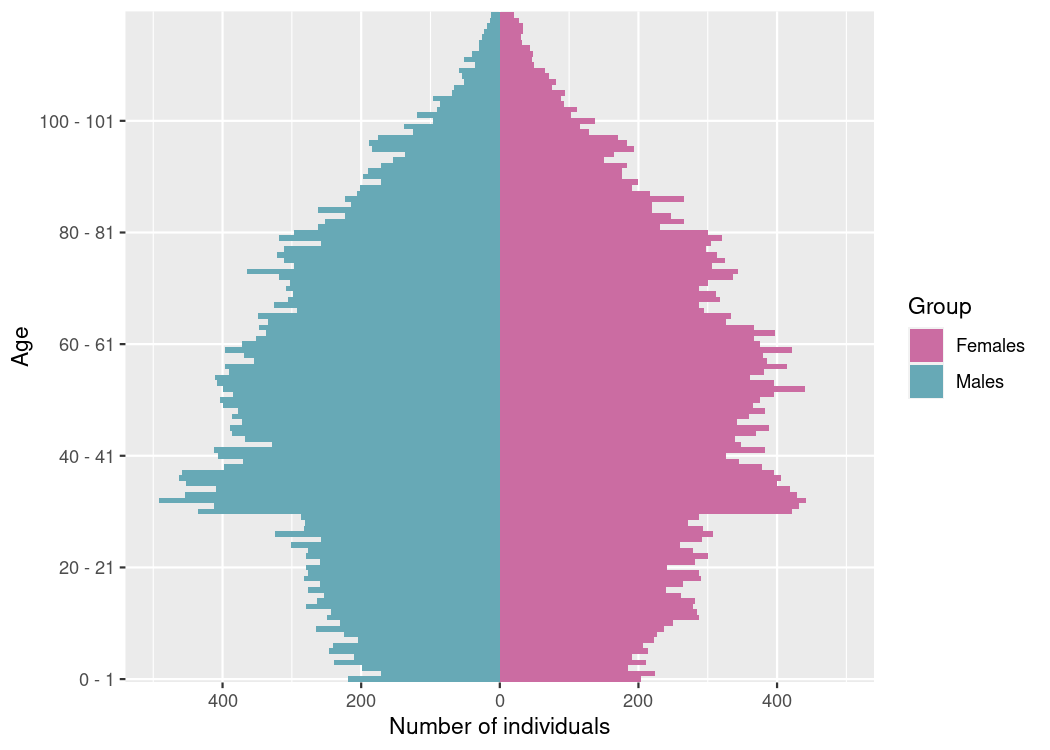
\includegraphics{main_plot_30-1} \end{center}

Mortality tables with compatibles with packages such as StMoMo can also be computed by with the functions \texttt{?death\_table} and \texttt{?exposure\_table}.

\begin{Shaded}
\begin{Highlighting}[]
\NormalTok{female\_pop }\OtherTok{\textless{}{-}}\NormalTok{ pop\_out[pop\_out}\SpecialCharTok{$}\NormalTok{male}\SpecialCharTok{==}\ConstantTok{FALSE}\NormalTok{, ]}
\NormalTok{Dxt }\OtherTok{\textless{}{-}} \FunctionTok{death\_table}\NormalTok{(female\_pop, }\AttributeTok{ages =} \DecValTok{85}\SpecialCharTok{:}\DecValTok{90}\NormalTok{, }\AttributeTok{period =} \DecValTok{20}\SpecialCharTok{:}\DecValTok{30}\NormalTok{)    }\CommentTok{\# Death table}
\NormalTok{Ext }\OtherTok{\textless{}{-}} \FunctionTok{exposure\_table}\NormalTok{(female\_pop, }\AttributeTok{ages =} \DecValTok{85}\SpecialCharTok{:}\DecValTok{90}\NormalTok{, }\AttributeTok{period =} \DecValTok{20}\SpecialCharTok{:}\DecValTok{30}\NormalTok{)}
\end{Highlighting}
\end{Shaded}

\hypertarget{simple-multithreading}{%
\subsubsection{Simple multithreading}\label{simple-multithreading}}

If there are \textbf{no interactions} between individuals, i.e.~if there are no events with intensity of class \texttt{interaction}, then the simulation can be parallelized easily by setting the optional parameter \texttt{multithreading} (\texttt{FALSE} by default) to \texttt{TRUE}:

\begin{Shaded}
\begin{Highlighting}[]
\NormalTok{sim\_out }\OtherTok{\textless{}{-}} \FunctionTok{popsim}\NormalTok{(model, pop, events\_bounds, params,}
                  \AttributeTok{age\_max =}\NormalTok{ a\_max, }\AttributeTok{time =} \DecValTok{30}\NormalTok{, }\AttributeTok{multithreading =} \ConstantTok{TRUE}\NormalTok{)}
\end{Highlighting}
\end{Shaded}

\begin{verbatim}
## duration_main_algorithm 
##                18101526
\end{verbatim}

By default, the number of threads is the number of concurrent threads supported by the available hardware implementation. The number of thread can be set manually with the optional argument \texttt{num\_threads} of \texttt{?popsim}.

\hypertarget{simulationswap}{%
\subsection{Simulation with swap events}\label{simulationswap}}

When there are swap events (individuals can change of characteristics), the dates of swap events and the changes of characteristics following each swap event should be recorded for each individual in the population, which is a memory intensive and computationally costly process.
To maintain efficient simulations in the presence of swap events, we propose the following solution.

\hypertarget{vector-of-times-in-popsim.}{%
\subsubsection{\texorpdfstring{Vector of times in \texttt{?popsim}.}{Vector of times in ?popsim.}}\label{vector-of-times-in-popsim.}}

In the presence of swap events, the argument \texttt{time} of \texttt{?popsim} should a vector of dates \((t_0,\dots, t_n)\). In this case, \texttt{popsim} returns in the object \texttt{population} a list of \(n\) population data frames representing the population at time \(t_1,\dots t_n\), simulated from the initial time \(t_0\).
For \(i=1\dots n\), the \(i\)th data frame describes individuals who lived in the population during the period \([t_0,t_i]\), with their characteristics at time \(t_i\).

\textbf{Examples} A population 100 thousand individuals (or particles) is generated, all born at time 0 and divided into two subgroups. Individuals can swap from subgroup 1 (resp. 2) to subgroup 2 (resp. 1) at rate 0.1 (resp. 0.3).

\begin{Shaded}
\begin{Highlighting}[]
\NormalTok{pop }\OtherTok{\textless{}{-}} \FunctionTok{data.frame}\NormalTok{(}\StringTok{"birth"} \OtherTok{=} \FunctionTok{rep}\NormalTok{(}\DecValTok{0}\NormalTok{,}\FloatTok{1e5}\NormalTok{), }\StringTok{"death"} \OtherTok{=} \FunctionTok{rep}\NormalTok{(}\ConstantTok{NA}\NormalTok{,}\FloatTok{1e5}\NormalTok{),}
                  \StringTok{"sub\_grp"} \OtherTok{=} \FunctionTok{sample}\NormalTok{(}\DecValTok{1}\SpecialCharTok{:}\DecValTok{2}\NormalTok{, }\FloatTok{1e5}\NormalTok{, }\AttributeTok{replace =} \ConstantTok{TRUE}\NormalTok{))}

\NormalTok{rates }\OtherTok{\textless{}{-}} \FunctionTok{list}\NormalTok{( }\AttributeTok{k12 =} \FloatTok{0.1}\NormalTok{, }\AttributeTok{k21=}\FloatTok{0.3}\NormalTok{)}
\CommentTok{\#Only swap events occur in the population}
\NormalTok{swap\_event }\OtherTok{\textless{}{-}} \FunctionTok{mk\_event\_individual}\NormalTok{(}\AttributeTok{type =} \StringTok{"swap"}\NormalTok{,}
                  \AttributeTok{intensity\_code =} \StringTok{"if (I.sub\_grp == 1) result = k12;}
\StringTok{                                    else result = k21;"}\NormalTok{,}
                  \AttributeTok{kernel\_code =} \StringTok{"I.sub\_grp = 3 {-} I.sub\_grp;"}\NormalTok{)}

\NormalTok{model\_swap }\OtherTok{\textless{}{-}} \FunctionTok{mk\_model}\NormalTok{(}\AttributeTok{characteristics =} \FunctionTok{get\_characteristics}\NormalTok{(pop),}
                       \AttributeTok{events =} \FunctionTok{list}\NormalTok{(swap\_event),}
                       \AttributeTok{parameters =}\NormalTok{ rates)}
\end{Highlighting}
\end{Shaded}

Then, the population is simulated from \(t_0=0\) to \(t_n =20\), and \texttt{popsim} returns a list of 20 data frames composed of the population at times \(t=1\dots 20\).

\begin{Shaded}
\begin{Highlighting}[]
\NormalTok{time\_vec }\OtherTok{\textless{}{-}} \DecValTok{0}\SpecialCharTok{:}\DecValTok{20}
\NormalTok{sim\_out }\OtherTok{\textless{}{-}}\FunctionTok{popsim}\NormalTok{(}\AttributeTok{model =}\NormalTok{ model\_swap, }\AttributeTok{population =}\NormalTok{ pop,}
                 \AttributeTok{events\_bounds =} \FunctionTok{c}\NormalTok{(}\StringTok{"swap"}\OtherTok{=}\FunctionTok{max}\NormalTok{(}\FunctionTok{unlist}\NormalTok{(rates))),}
                 \AttributeTok{parameters =}\NormalTok{  rates,}
                 \AttributeTok{time =}\NormalTok{ time\_vec,}
                 \AttributeTok{multithreading =} \ConstantTok{TRUE}\NormalTok{)}
\end{Highlighting}
\end{Shaded}

The model is an ergodic two states continuous time Markov chain with stationary distribution \((p_1,p_2)=(0,75,0.25)\). The figure below illustrates the convergence of the probability to be in subgroup 1 to \(p_1\)

\begin{Shaded}
\begin{Highlighting}[]
\NormalTok{pop\_size }\OtherTok{\textless{}{-}} \FunctionTok{nrow}\NormalTok{(pop)}
\CommentTok{\# Mean number of individuals in subgroup 1 at each time:}
\NormalTok{p\_1\_t }\OtherTok{\textless{}{-}} \FunctionTok{lapply}\NormalTok{(sim\_out}\SpecialCharTok{$}\NormalTok{population, }\ControlFlowTok{function}\NormalTok{(pop\_df)\{}
                      \FunctionTok{return}\NormalTok{(}\FunctionTok{nrow}\NormalTok{(}\FunctionTok{subset}\NormalTok{(pop\_df, sub\_grp}\SpecialCharTok{==}\DecValTok{1}\NormalTok{))}\SpecialCharTok{/}\NormalTok{pop\_size)}
\NormalTok{                \})}
\end{Highlighting}
\end{Shaded}

\begin{center}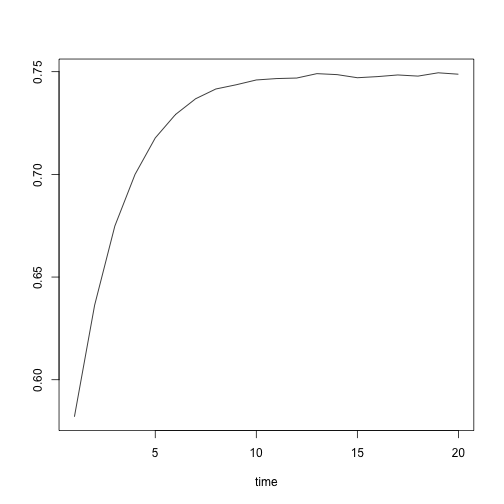
\includegraphics{main_prob_subgroup1-1} \end{center}

This example shows that IBMPopSIm can also be used to simulated continuous time Markov Chain with finite state space.

\hypertarget{individual-life-courses}{%
\subsubsection{Individual life courses}\label{individual-life-courses}}

It is possible to isolate the individuals' life course, by setting the optional argument \texttt{with\_id} of \texttt{?mk\_model} to \texttt{TRUE}. In this case, a new characteristic called \texttt{id} is automatically added to the population (if not already defined), identifying each individual with a unique integer.

\begin{Shaded}
\begin{Highlighting}[]
\NormalTok{model\_swap\_id }\OtherTok{\textless{}{-}} \FunctionTok{mk\_model}\NormalTok{(}\AttributeTok{characteristics =}  \FunctionTok{get\_characteristics}\NormalTok{(pop),}
                          \AttributeTok{events =} \FunctionTok{list}\NormalTok{(swap\_event),}
                          \AttributeTok{parameters =}\NormalTok{ rates,}
                          \AttributeTok{with\_id =} \ConstantTok{TRUE}\NormalTok{)}
\DocumentationTok{\#\# [1] "add \textquotesingle{}id\textquotesingle{} as individual attributes"}
\end{Highlighting}
\end{Shaded}

\begin{Shaded}
\begin{Highlighting}[]
\NormalTok{sim\_out\_id }\OtherTok{\textless{}{-}}\FunctionTok{popsim}\NormalTok{(}\AttributeTok{model =}\NormalTok{ model\_swap\_id,}
                    \AttributeTok{population =}\NormalTok{ pop,}
                    \AttributeTok{parameters =}\NormalTok{ rates,}
                    \AttributeTok{events\_bounds =} \FunctionTok{c}\NormalTok{(}\StringTok{"swap"}\OtherTok{=}\FloatTok{0.3}\NormalTok{),}
                    \AttributeTok{time =} \FunctionTok{seq}\NormalTok{(}\DecValTok{0}\NormalTok{,}\DecValTok{5}\NormalTok{, }\AttributeTok{by=}\DecValTok{1}\NormalTok{),}
                    \AttributeTok{multithreading =} \ConstantTok{TRUE}\NormalTok{)}
\DocumentationTok{\#\# [1] "Add \textquotesingle{}id\textquotesingle{} attributes to the population."}
\DocumentationTok{\#\# Simulation on  [0, 1]  [1, 2]  [2, 3]  [3, 4]  [4, 5]}
\end{Highlighting}
\end{Shaded}

\begin{Shaded}
\begin{Highlighting}[]
\FunctionTok{head}\NormalTok{(sim\_out\_id}\SpecialCharTok{$}\NormalTok{population[[}\DecValTok{1}\NormalTok{]])}
\DocumentationTok{\#\#   id birth death sub\_grp}
\DocumentationTok{\#\# 1  1     0    NA       1}
\DocumentationTok{\#\# 2  9     0    NA       2}
\DocumentationTok{\#\# 3 17     0    NA       1}
\DocumentationTok{\#\# 4 25     0    NA       2}
\DocumentationTok{\#\# 5 33     0    NA       2}
\DocumentationTok{\#\# 6 41     0    NA       1}
\end{Highlighting}
\end{Shaded}

These data frames can be merged into a single data frame summarizing the life course of each individual, by calling the function \texttt{merge\_pop\_withid}.

\begin{Shaded}
\begin{Highlighting}[]
\NormalTok{pop\_list }\OtherTok{\textless{}{-}}\NormalTok{ sim\_out\_id}\SpecialCharTok{$}\NormalTok{population}
\NormalTok{pop\_merge }\OtherTok{\textless{}{-}} \FunctionTok{merge\_pop\_withid}\NormalTok{(pop\_list, }\AttributeTok{chars\_tracked=}\StringTok{\textquotesingle{}sub\_grp\textquotesingle{}}\NormalTok{)}
\FunctionTok{head}\NormalTok{(pop\_merge)}
\DocumentationTok{\#\#      id birth death sub\_grp\_1 sub\_grp\_2 sub\_grp\_3 sub\_grp\_4 sub\_grp\_5}
\DocumentationTok{\#\# 1     1     0    NA         1         1         1         1         1}
\DocumentationTok{\#\# 2 32769     0    NA         2         1         2         2         2}
\DocumentationTok{\#\# 3 65537     0    NA         1         1         1         2         2}
\DocumentationTok{\#\# 4 98305     0    NA         2         1         1         2         1}
\DocumentationTok{\#\# 5 31074     0    NA         2         2         2         1         1}
\DocumentationTok{\#\# 6 63842     0    NA         1         1         1         1         1}
\end{Highlighting}
\end{Shaded}

Each line of \texttt{pop\_merge} corresponds to the life course of one individual. However, the population is only represented at time \(t=0,1..,5\), and this data frame doesn't account for exact swap event times or multiple swap events that occurred between between two time steps.

\hypertarget{cppessentials}{%
\section{C++ essentials}\label{cppessentials}}

The arguments \texttt{intensity\_code}, \texttt{interaction\_code} and \texttt{kernel\_code} of the events functions must contain some C++ code given by the user. You don't need to be a C++ guru to write the few instructions needed. These functions should use very little C++ syntax. They are essentially arithmetic or logical operations, tests and calls to predefined functions, which we give an overview below.

For code efficiency, you should not allocate memory in these functions (no \texttt{new}) or use type containers (\texttt{std::vector}, \texttt{std::list}, \ldots). If you think you need to allocate memory, consider as parameter an R vector that will be mapped via \texttt{arma::vector} (see below), or declare the variable as \texttt{static}.
Also, it should not be necessary to make a loop. Keep in mind that these functions should be fast.

There are no C++ language restrictions so you can use all the functions of the standard C++11 library. However we detail in this section some functions that should be sufficient. For more details on C++ and Rcpp we recommend:

\begin{itemize}
\tightlist
\item
  \href{https://www.cplusplus.com/doc/tutorial/}{C++ tutorial}
\item
  \href{http://dirk.eddelbuettel.com/code/rcpp.html}{Rcpp} and \href{http://dirk.eddelbuettel.com/code/rcpp.armadillo.html}{RcppArmadillo}
\item
  \href{https://teuder.github.io/rcpp4everyone_en/}{Rcpp for everyone}
\end{itemize}

\hypertarget{c-syntax}{%
\subsection{C++ syntax}\label{c-syntax}}

\begin{itemize}
\tightlist
\item
  Each statement must be ended by a semicolon.
\item
  Single-line comments start with two forward slashes \texttt{//}.
\item
  To create a variable, you must specify the type and assign it a value (type variable = value;). Here some examples:
\end{itemize}

\begin{verbatim}
int myNum = 5;               // Integer (whole number without decimals)
double myFloatNum = 5.99;    // Floating point number (with decimals)
char myLetter = 'D';         // Character
bool myBoolean = true;       // Boolean (true or false)
\end{verbatim}

\begin{itemize}
\tightlist
\item
  \texttt{bool} data type can take the values \texttt{true} (1) or \texttt{false} (0).
\item
  C++ supports the usual logical conditions from mathematics:

  \begin{itemize}
  \tightlist
  \item
    Less than: \texttt{a\ \textless{}\ b}
  \item
    Less than or equal to: \texttt{a\ \textless{}=\ b}
  \item
    Greater than: \texttt{a\ \textgreater{}\ b}
  \item
    Greater than or equal to: \texttt{a\ \textgreater{}=\ b}
  \item
    Equal to \texttt{a\ ==\ b}
  \item
    Not Equal to: \texttt{a\ !=\ b}
  \end{itemize}
\item
  The logical operators are: \texttt{!}, \texttt{\&\&}, \texttt{\textbar{}\textbar{}}
\item
  The arithmetic operators are: \texttt{+}, \texttt{-}, \texttt{*}, \texttt{/}, \texttt{\%}
\item
  Compound assignment: \texttt{+=}, \texttt{-=}, \texttt{*=}, \texttt{/=}, \texttt{\%=}
\item
  Increment and decrement: \texttt{++}, \texttt{-\/-}
\item
  Conditional ternary operator: \texttt{?\ :}
  The conditional operator evaluates an expression, returning one value if that expression evaluates to \texttt{true}, and a different one if the expression evaluates as \texttt{false}. Its syntax is:
\end{itemize}

\begin{verbatim}
condition ? result1; : result2;
\end{verbatim}

\begin{itemize}
\tightlist
\item
  Use the \texttt{if}, \texttt{else\ if}, \texttt{else} statements to specify a block of C++ code to be executed if one or more conditions are or not \texttt{true}.
\end{itemize}

\begin{verbatim}
if (condition1) {
  // block of code to be executed if condition1 is true
} else if (condition2) {
  // block of code to be executed if the condition1 is false and condition2 is true
} else {
  // block of code to be executed if the condition1 is false and condition2 is false
}
\end{verbatim}

\begin{itemize}
\tightlist
\item
  The syntax of the switch statement is a bit peculiar. Its purpose is to check for a value among a number of possible constant expressions. It is something similar to concatenating \texttt{if-else} statements, but limited to constant expressions. Its most typical syntax is:
\end{itemize}

\begin{verbatim}
switch (expression)
{
  case constant1:
     group-of-statements-1;
     break;
  case constant2:
     group-of-statements-2;
     break;
  .
  .
  .
  default:
     default-group-of-statements
}
\end{verbatim}

It works in the following way: switch evaluates expression and checks if it is equivalent to \texttt{constant1}; if it is, it executes \texttt{group-of-statements-1} until it finds the \texttt{break} statement. When it finds this break statement, the program jumps to the end of the entire switch statement (the closing brace).

\begin{itemize}
\tightlist
\item
  When you know exactly how many times you want to loop through a block of code, use the \texttt{for} loop.
\end{itemize}

\begin{verbatim}
for (statement 1; statement 2; statement 3) {
  // code block to be executed
}
\end{verbatim}

\begin{itemize}
\tightlist
\item
  The while loop loops through a block of code as long as a specified condition is true.
\end{itemize}

\begin{verbatim}
while (condition) {
  // code block to be executed
}
\end{verbatim}

For more details we recommend a few pages of \href{https://www.cplusplus.com/}{www.cplusplus.com} about:

\begin{itemize}
\tightlist
\item
  \href{https://www.cplusplus.com/doc/tutorial/variables/}{Variables}
\item
  \href{https://www.cplusplus.com/doc/tutorial/operators/}{Operators}
\item
  \href{https://www.cplusplus.com/doc/tutorial/control/}{Statements}
\end{itemize}

\hypertarget{usual-numeric-functions}{%
\subsection{Usual numeric functions}\label{usual-numeric-functions}}

The most popular functions of the \texttt{cmath} library, which is included in the package, are the following:

\begin{itemize}
\tightlist
\item
  Exponential and logarithm functions: \texttt{exp(x)}, \texttt{log(x)} (natural logarithm)
\item
  Trigonometric functions: \texttt{cos(x)}, \texttt{sin(x)}, \texttt{tan(x)}
\item
  Power functions: \texttt{pow(x,\ a)} meaning \(x^a\) and \texttt{sqrt(x)} meaning \(\sqrt{x}\)
\item
  Absolute value: \texttt{abs(x)}
\item
  Truncation functions: \texttt{ceil(x)} meaning \(\lceil x \rceil\) and \texttt{floor(x)} meaning \(\lfloor x \rfloor\)
\item
  Bivariate functions: \texttt{max(x,\ y)} and \texttt{min(x,y)}
\end{itemize}

Note that these functions are not vectorial, the arguments \texttt{x} and \texttt{y} must be scalar. If the user wants to call some other functions of \texttt{cmath} not listed in the table, this is possible by adding the prefix \texttt{std::} to the name of the function (scope resolution operator \texttt{::} to access to functions declared in namespace standard \texttt{std}).

\hypertarget{cppcharacteristics}{%
\subsection{Individuals characteristics and model parameters: link between R and C++}\label{cppcharacteristics}}

To facilitate the model creation, the individuals' characteristics and a list model parameters can be declared in the R environment and used in the C++ code.

The data shared between the R environment and the C++ code are:

\begin{itemize}
\tightlist
\item
  The characteristics of the individuals which must be atomic (Boolean, scalar or character).
\item
  The model parameters: a list of variables of type:

  \begin{itemize}
  \tightlist
  \item
    Atomic, vector or matrix.
  \item
    Predefined real functions of one variable, or list of such functions.
  \item
    Piecewise real function of two variables, of list of such.
  \end{itemize}
\end{itemize}

\hypertarget{atomic-types-characteristics-and-parameters}{%
\subsubsection{Atomic types (characteristics and parameters)}\label{atomic-types-characteristics-and-parameters}}

Here is the conversion table used between the atomic types of R and C++.

\begin{longtable}[]{@{}ll@{}}
\toprule()
C++ type & R type \\
\midrule()
\endhead
bool & \texttt{logical} \\
int & \texttt{integer} \\
double & \texttt{double} \\
char & \texttt{character} \\
\bottomrule()
\end{longtable}

\textbf{Individuals characteristics}

The characteristics of an individual are defined by a named character vector containing the name of the characteristic and the associated C++ type. The function \texttt{?get\_characteristics} provides a way to extract the characteristics from a population data frame.

\begin{Shaded}
\begin{Highlighting}[]
\FunctionTok{library}\NormalTok{(IBMPopSim)}
\NormalTok{pop }\OtherTok{\textless{}{-}}\NormalTok{ IBMPopSim}\SpecialCharTok{::}\NormalTok{EW\_popIMD\_14}\SpecialCharTok{$}\NormalTok{sample}
\FunctionTok{get\_characteristics}\NormalTok{(pop)}
\DocumentationTok{\#\#   male    IMD }
\DocumentationTok{\#\# "bool"  "int"}
\end{Highlighting}
\end{Shaded}

The requires \texttt{birth} and \texttt{death} characteristics are of type \texttt{double}.

\textbf{Atomic model parameters}

The model parameters are given by a named list of R objects. We recall that the type of an R object can be determined by calling the \texttt{?typeof} function. Atomic objects declared as model parameters can be directly used in the C++ code.\\
In the example below, the variable \texttt{code} contains simple C++ instructions depending on the parameters defined in \texttt{params}. The \texttt{summary} of the model \texttt{mod} gives useful information on the types of characteristics and parameters used in C++ code.

\begin{Shaded}
\begin{Highlighting}[]
\NormalTok{params }\OtherTok{\textless{}{-}} \FunctionTok{list}\NormalTok{(}\StringTok{"lambda"} \OtherTok{=} \FloatTok{0.02}\NormalTok{, }\StringTok{"alpha"} \OtherTok{=} \FloatTok{0.4}\NormalTok{, }\StringTok{"mu"} \OtherTok{=} \FunctionTok{as.integer}\NormalTok{(}\DecValTok{2}\NormalTok{))}
\NormalTok{code }\OtherTok{\textless{}{-}} \StringTok{"result = lambda + alpha * (age(I, t) + mu);"}
\NormalTok{event\_birth }\OtherTok{\textless{}{-}} \FunctionTok{mk\_event\_individual}\NormalTok{(}\StringTok{"birth"}\NormalTok{, }\AttributeTok{intensity\_code =}\NormalTok{ code)}
\NormalTok{mod }\OtherTok{\textless{}{-}} \FunctionTok{mk\_model}\NormalTok{(}\FunctionTok{get\_characteristics}\NormalTok{(pop), }\AttributeTok{events =} \FunctionTok{list}\NormalTok{(}\StringTok{"birth"} \OtherTok{=}\NormalTok{ event\_birth), }
                \AttributeTok{parameters =}\NormalTok{ params, }\AttributeTok{with\_compilation =} \ConstantTok{FALSE}\NormalTok{)}
\FunctionTok{summary}\NormalTok{(mod)}
\DocumentationTok{\#\# Events:}
\DocumentationTok{\#\# \#1: individual event of type birth}
\DocumentationTok{\#\# {-}{-}{-}{-}{-}{-}{-}{-}{-}{-}{-}{-}{-}{-}{-}{-}{-}{-}{-}{-}{-}{-}{-}{-}{-}{-}{-}{-}{-}{-}{-}{-}{-}{-}{-}{-}{-}{-}{-} }
\DocumentationTok{\#\# Individual description:}
\DocumentationTok{\#\# names:  birth death male IMD }
\DocumentationTok{\#\# R types:  double double logical integer }
\DocumentationTok{\#\# C types:  double double bool int}
\DocumentationTok{\#\# {-}{-}{-}{-}{-}{-}{-}{-}{-}{-}{-}{-}{-}{-}{-}{-}{-}{-}{-}{-}{-}{-}{-}{-}{-}{-}{-}{-}{-}{-}{-}{-}{-}{-}{-}{-}{-}{-}{-} }
\DocumentationTok{\#\# R parameters available in C++ code:}
\DocumentationTok{\#\# names:  lambda alpha mu }
\DocumentationTok{\#\# R types:  double double integer }
\DocumentationTok{\#\# C types:  double double int}
\end{Highlighting}
\end{Shaded}

\hypertarget{cpparmadillo}{%
\subsubsection{Vectors and matrices (model parameters)}\label{cpparmadillo}}

Two of the possible model parameters types given in the argument \texttt{parameters} of the \texttt{?mk\_model} function are R vectors and R matrices. We call R vector a \texttt{numeric} of length at least 2. These types are converted, using the \href{http://dirk.eddelbuettel.com/code/rcpp.armadillo.html}{RcppArmadillo library}, in C++ \href{http://arma.sourceforge.net/}{Armadillo} types, \texttt{arma::vec} and \texttt{arma::matrix} respectively.

The classes \texttt{arma::vec} and \texttt{arma::matrix} are rich and easy-to-use implementations of one-dimensional and two-dimensional arrays. To access to individual elements of an array, use the operator \texttt{()} (or \texttt{{[}{]}} in dimension 1).

\begin{itemize}
\tightlist
\item
  \texttt{(n)} or \texttt{{[}n{]}} for \texttt{arma::vec}, access the n-th element.
\item
  \texttt{(i,j)} for \texttt{arma::matrix}, access the element stored at the \(i\)-th row and \(j\)-th column.
\end{itemize}

\textbf{Warning:} The first element of the array is indexed by subscript of 0 (in each dimension).

Another standard way (in C++) to access elements is to used iterators. An iterator is an object that, pointing to some element in a range of elements, has the ability to iterate through the elements of that range using a set of operators (see \href{https://teuder.github.io/rcpp4everyone_en/290_iterator.html}{more details on iterators}).

Let \texttt{v} be a an object of type \texttt{arma::vec} and A be a an object of type \texttt{arma::matrix}. Here we show how to get the begin and the end iterators of these objects.

\begin{itemize}
\tightlist
\item
  \texttt{v.begin()}: iterator pointing to the begin of \texttt{v}
\item
  \texttt{v.end()}: iterator pointing to the end of \texttt{v}
\item
  \texttt{A.begin\_row(i)}: iterator pointing to the first element of row \texttt{i}
\item
  \texttt{A.end\_row(i)}: iterator pointing to the last element of row \texttt{i}
\item
  \texttt{A.begin\_col(i)}: iterator pointing to the first element of column \texttt{i}
\item
  \texttt{A.end\_col(i)}: iterator pointing to the last element of column \texttt{i}
\end{itemize}

\hypertarget{cppIBMfunctions}{%
\subsubsection{Predefined functions (model parameters)}\label{cppIBMfunctions}}

To facilitate the implementation of intensity functions and kernel code, R functions have been predefined in \texttt{IBMPopSim}, which can be defined as model parameters and then called in the C++ code. The goal is to make their use as transparent as possible.

\hypertarget{real-functions-of-one-variable}{%
\paragraph{Real functions of one variable}\label{real-functions-of-one-variable}}

Here is a list of such functions that can be defined as a R object and called from R and C++.

\begin{itemize}
\tightlist
\item
  \texttt{stepfun}: Step function.
\item
  \texttt{linfun}: Linear interpolation function.
\item
  \texttt{gompertz}: Gompertz--Makeham intensity function.
\item
  \texttt{weibull}: Weibull density function.
\item
  \texttt{piecewise\_x}: Piecewise real function.
\end{itemize}

See the reference manual for mathematical definitions of these functions (\texttt{?stepfun}).\\
Once the model is created, these predefined functions are transformed into C++ functions, identified as \texttt{function\_x}.

We illustrate below some examples of the use of these functions:

\begin{enumerate}
\def\labelenumi{\arabic{enumi}.}
\tightlist
\item
  We define \texttt{dr} a \texttt{stepfun} depending on some values in \texttt{EW\_pop\_14\$rates}. Note that this function applies to an age \texttt{a}.
\end{enumerate}

\begin{Shaded}
\begin{Highlighting}[]
\NormalTok{dr }\OtherTok{\textless{}{-}} \FunctionTok{with}\NormalTok{(EW\_pop\_14}\SpecialCharTok{$}\NormalTok{rates,}
           \FunctionTok{stepfun}\NormalTok{(}\AttributeTok{x =}\NormalTok{ death\_male[,}\StringTok{"age"}\NormalTok{], }\AttributeTok{y =} \FunctionTok{c}\NormalTok{(}\DecValTok{0}\NormalTok{, death\_male[,}\StringTok{"value"}\NormalTok{])))}
\FunctionTok{plot}\NormalTok{(dr, }\AttributeTok{xlab=}\StringTok{"age"}\NormalTok{, }\AttributeTok{ylab=}\StringTok{"dr"}\NormalTok{, }\AttributeTok{main=}\StringTok{"Example of step function"}\NormalTok{)}
\end{Highlighting}
\end{Shaded}

\begin{center}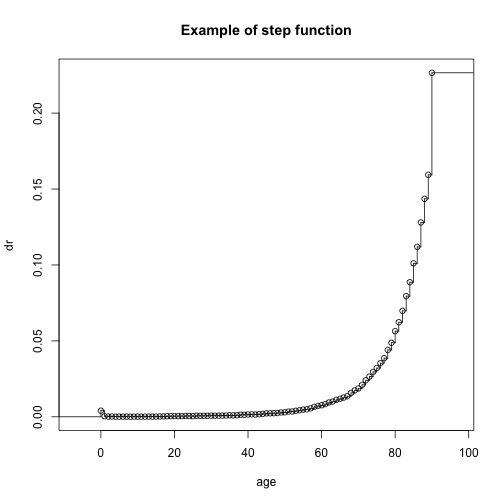
\includegraphics{plot_stepfun-1} \end{center}

We can also initialize a piecewise real function \texttt{f} defined by the function \texttt{dr} before age 80, and by a Gompertz-Makeham intensity function for ages after 80.

\begin{Shaded}
\begin{Highlighting}[]
\NormalTok{f }\OtherTok{\textless{}{-}} \FunctionTok{piecewise\_x}\NormalTok{(}\DecValTok{80}\NormalTok{, }\FunctionTok{list}\NormalTok{(dr, }\FunctionTok{gompertz}\NormalTok{(}\FloatTok{0.00006}\NormalTok{, }\FloatTok{0.085}\NormalTok{)))}
\NormalTok{x }\OtherTok{\textless{}{-}} \FunctionTok{seq}\NormalTok{(}\DecValTok{40}\NormalTok{, }\DecValTok{110}\NormalTok{)}
\FunctionTok{plot}\NormalTok{(x, }\FunctionTok{sapply}\NormalTok{(x, f), }\AttributeTok{xlab=}\StringTok{"age"}\NormalTok{, }\AttributeTok{ylab=}\StringTok{"f"}\NormalTok{, }\AttributeTok{main=}\StringTok{"Example of piecewise function"}\NormalTok{)}
\end{Highlighting}
\end{Shaded}

\begin{center}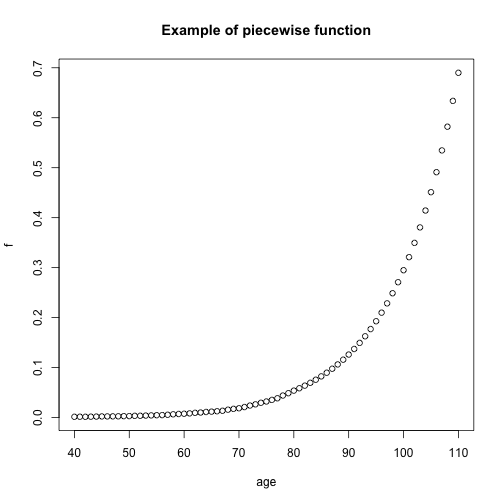
\includegraphics{plot_piecewise-1} \end{center}

\begin{enumerate}
\def\labelenumi{\arabic{enumi}.}
\setcounter{enumi}{1}
\tightlist
\item
  Once a function has been created and defined as model parameter, a model depending on the function can be defined. For example we use in the model below the \texttt{stepfun} \texttt{dr} as a model parameter named \texttt{rate}. The function is used to defined the intensity of death events in the model.
  s
\end{enumerate}

\begin{Shaded}
\begin{Highlighting}[]
\NormalTok{params }\OtherTok{\textless{}{-}} \FunctionTok{list}\NormalTok{(}\StringTok{"rate"} \OtherTok{=}\NormalTok{ dr)}
\NormalTok{event }\OtherTok{\textless{}{-}} \FunctionTok{mk\_event\_individual}\NormalTok{(}\StringTok{"death"}\NormalTok{, }\AttributeTok{intensity\_code =} \StringTok{"result = rate(age(I, t));"}\NormalTok{)}
\NormalTok{mod }\OtherTok{\textless{}{-}} \FunctionTok{mk\_model}\NormalTok{(}\FunctionTok{get\_characteristics}\NormalTok{(pop), }\AttributeTok{events =} \FunctionTok{list}\NormalTok{(}\StringTok{"death"} \OtherTok{=}\NormalTok{ event), }
                \AttributeTok{parameters =}\NormalTok{ params, }\AttributeTok{with\_compilation =} \ConstantTok{FALSE}\NormalTok{)}
\FunctionTok{summary}\NormalTok{(mod)}
\DocumentationTok{\#\# Events:}
\DocumentationTok{\#\# \#1: individual event of type death}
\DocumentationTok{\#\# {-}{-}{-}{-}{-}{-}{-}{-}{-}{-}{-}{-}{-}{-}{-}{-}{-}{-}{-}{-}{-}{-}{-}{-}{-}{-}{-}{-}{-}{-}{-}{-}{-}{-}{-}{-}{-}{-}{-} }
\DocumentationTok{\#\# Individual description:}
\DocumentationTok{\#\# names:  birth death male IMD }
\DocumentationTok{\#\# R types:  double double logical integer }
\DocumentationTok{\#\# C types:  double double bool int}
\DocumentationTok{\#\# {-}{-}{-}{-}{-}{-}{-}{-}{-}{-}{-}{-}{-}{-}{-}{-}{-}{-}{-}{-}{-}{-}{-}{-}{-}{-}{-}{-}{-}{-}{-}{-}{-}{-}{-}{-}{-}{-}{-} }
\DocumentationTok{\#\# R parameters available in C++ code:}
\DocumentationTok{\#\# names:  rate }
\DocumentationTok{\#\# R types:  closure }
\DocumentationTok{\#\# C types:  function\_x}
\end{Highlighting}
\end{Shaded}

\begin{enumerate}
\def\labelenumi{\arabic{enumi}.}
\setcounter{enumi}{2}
\tightlist
\item
  After compilation, the parameter \texttt{rate} can actually be replaced by any function of type \texttt{function\_x}. For example you can call
\end{enumerate}

\begin{verbatim}
popsim(mod, pop, params = list("rate" = dr), age_max = 120, 
       events_bounds = c("death" = dr(age_max)), time = 10)
\end{verbatim}

as well as

\begin{verbatim}
popsim(mod, pop, params = list("rate" = f), age_max = 120, 
       events_bounds = c("death" = f(age_max)), time = 10)
\end{verbatim}

\hypertarget{piecewise-real-functions-of-two-variables}{%
\paragraph{Piecewise real functions of two variables}\label{piecewise-real-functions-of-two-variables}}

In the C++ code these R functions declared with \texttt{?piecewise\_xy} are identified as \texttt{function\_xy} functions. See \texttt{?piecewise\_xy} for mathematical definition. This function allows to easily define a step function that depend on age and time.

\hypertarget{list-of-functions}{%
\paragraph{List of functions}\label{list-of-functions}}

As parameter you can use a list of functions. All R functions in the list must be of the same C++ type: either \texttt{function\_x} or \texttt{function\_xy}. In C++ code the list of functions is replaced by a \texttt{std::vector} of \texttt{function\_x} or \texttt{function\_xy} (with first element indexed by 0).

\hypertarget{randomvar}{%
\subsection{Random variables}\label{randomvar}}

We use the following notations to describe the available C++ random distributions, which can be used in the C++ intensity and kernel codes.

\begin{itemize}
\item
  \(\mathcal{U}(a,b)\) : Uniform distribution on \([a, b]\) with \(a < b\)
\item
  \(\mathcal{E}(\lambda)\) : Exponential distribution, \(\lambda > 0\)
\item
  \(\mathcal{N}(\mu,\sigma)\) : Gaussian distribution, \(\mu, \sigma \in \mathbf{R}\)
\item
  \(\mathrm{Pois}(\lambda)\): Poisson distribution, \(\lambda > 0\)
\item
  \(\Gamma(\alpha, \beta)\): Gamma distribution, \(\alpha > 0\), \(\beta > 0\)
\item
  \(\mathrm{Weib}(a, b)\): Weibull distribution, \(a > 0\), \(b > 0\)
\item
  \(\mathcal{U}\{a, b\}\): Discrete uniform distribution on \(\{a, a+1, \dots, b\}\) with \(a < b\)
\item
  \(\mathcal{B}(p)\): Bernoulli distribution, the probability of success is \(p \in (0,1)\)
\item
  \(\mathcal{B}(n, p)\): Binomial distribution \(n \ge 1\), \(p \in (0,1)\)
\item
  \(\mathcal{D}_n\) : Discrete distribution with values in \(\{ 0, \dots, n-1 \}\) and with probabilities \(\{p_0, \dots, p_{n-1}\}\).
\end{itemize}

In the table below we show how to call them, which means how to make independent realizations of these random variables, and we give the reference to the C++ corresponding function of the \href{http://www.cplusplus.com/reference/random/}{random library} hidden in this call.

\begin{longtable}[]{@{}
  >{\raggedright\arraybackslash}p{(\columnwidth - 4\tabcolsep) * \real{0.3333}}
  >{\raggedright\arraybackslash}p{(\columnwidth - 4\tabcolsep) * \real{0.3333}}
  >{\raggedright\arraybackslash}p{(\columnwidth - 4\tabcolsep) * \real{0.3333}}@{}}
\toprule()
\begin{minipage}[b]{\linewidth}\raggedright
Function call
\end{minipage} & \begin{minipage}[b]{\linewidth}\raggedright
Meaning
\end{minipage} & \begin{minipage}[b]{\linewidth}\raggedright
C++ \href{http://www.cplusplus.com/reference/random/}{\texttt{random}} internal function
\end{minipage} \\
\midrule()
\endhead
CUnif(\(a=0, b=1\)) & \(\mathcal{U}(a,b)\) & \href{http://www.cplusplus.com/reference/random/uniform_real_distribution/}{\texttt{uniform\_real\_distribution\textless{}double\textgreater{}}} \\
CExp(\(\lambda=1\)) & \(\mathcal{E}(\lambda)\) & \href{http://www.cplusplus.com/reference/random/exponential_distribution/}{\texttt{exponential\_distribution\textless{}double\textgreater{}}} \\
CNorm(\(\mu=0, \sigma=1\)) & \(\mathcal{N}(\mu,\sigma)\) & \href{http://www.cplusplus.com/reference/random/normal_distribution/}{\texttt{normal\_distribution\textless{}double\textgreater{}}} \\
CPoisson(\(\lambda=1\)) & \(\mathrm{Pois}(\lambda)\) & \href{http://www.cplusplus.com/reference/random/poisson_distribution/}{\texttt{poisson\_distribution\textless{}unsigned\textgreater{}}} \\
CGamma(\(\alpha=1, \beta=1\)) & \(\Gamma(\alpha,\beta)\) & \href{http://www.cplusplus.com/reference/random/gamma_distribution/}{\texttt{gamma\_distribution\textless{}double\textgreater{}}} \\
CWeibull(\(a=1\), \(b=1\)) & \(\mathrm{Weib}(a,b)\) & \href{http://www.cplusplus.com/reference/random/weibull_distribution/}{\texttt{weibull\_distribution\textless{}double\textgreater{}}} \\
CUnifInt(\(a=0, b=2^{31}-1\)) & \(\mathcal{U}\{a,b\}\) & \href{http://www.cplusplus.com/reference/random/uniform_int_distribution/}{\texttt{uniform\_int\_distribution\textless{}int\textgreater{}}} \\
CBern(\(p=0.5\)) & \(\mathcal{B}(p)\) & \href{http://www.cplusplus.com/reference/random/bernoulli_distribution/}{\texttt{bernoulli\_distribution}} \\
CBinom(\(n=1, p=0.5\)) & \(\mathcal{B}(n,p)\) & \href{http://www.cplusplus.com/reference/random/binomial_distribution/}{\texttt{binomial\_distribution\textless{}int\textgreater{}}} \\
CDiscrete(\texttt{p\_begin}, \texttt{p\_end}) & \(\mathcal{D}_n\) & \href{http://www.cplusplus.com/reference/random/discrete_distribution/}{\texttt{discrete\_distribution\textless{}int\textgreater{}}} \\
\bottomrule()
\end{longtable}

In the discrete distribution call \texttt{CDiscrete(p\_begin,\ p\_end)}, the arguments \texttt{p\_begin} and \texttt{p\_end} represent the iterators to the begin and to the end of an array which contains \(\{p_0, \dots, p_{n-1}\}\). Note that the use of iterators is a convenient and fast way to access a column or row of a matrix \texttt{arma::mat}.

\hypertarget{references}{%
\section{References}\label{references}}

\hypertarget{refs}{}
\begin{CSLReferences}{1}{0}
\leavevmode\vadjust pre{\hypertarget{ref-boumezoued2016}{}}%
Boumezoued, Alexandre. 2016. {``Approches Micro-Macro Des Dynamiques de Populations h{é}t{é}rog{è}nes Structur{é}es Par {â}ge. Application Aux Processus Auto-Excitants Et {à} La d{é}mographie.''}

\leavevmode\vadjust pre{\hypertarget{ref-MR2562651}{}}%
Ferrière, Régis, and Viet Chi Tran. 2009. {``Stochastic and Deterministic Models for Age-Structured Populations with Genetically Variable Traits.''} \emph{ESAIM Proc. C{ANUM} 2008} 27 (4): 289--310.

\leavevmode\vadjust pre{\hypertarget{ref-MELEARD2004}{}}%
Fournier, Nicolas, and Sylvie Méléard. 2004. {``{A microscopic probabilistic description of a locally regulated population and macroscopic approximations}.''} \emph{Annals of Applied Probability} 14 (4): 1880--1919.

\end{CSLReferences}
  </div>

  <div class="col-md-3 hidden-xs hidden-sm" id="pkgdown-sidebar">

        <nav id="toc" data-toggle="toc"><h2 data-toc-skip>Contents</h2>
    </nav>
      </div>

</div>



      <footer><div class="copyright">
  <p></p><p>Developed by Daphné Giorgi, Sarah Kaakai, Vincent Lemaire.</p>
</div>

<div class="pkgdown">
  <p></p><p>Site built with <a href="https://pkgdown.r-lib.org/" class="external-link">pkgdown</a> 2.0.6.</p>
</div>

      </footer></div>

  


  

  </body></html>
